\documentclass[12pt, oneside]{book}

\usepackage[T2A]{fontenc}			% кодировка
\usepackage[utf8]{inputenc}			% кодировка исходного текста
\usepackage[english,russian]{babel}	% локализация и переносы

\usepackage{amsmath}
\usepackage{amsthm, mathrsfs, mathtools, amssymb}
\usepackage{enumitem}

\usepackage{epigraph}

\usepackage{geometry}
\geometry{verbose,a4paper,tmargin=2cm,bmargin=2cm,lmargin=2.5cm,rmargin=1.5cm}

%\usepackage{showframe}

\usepackage{accents}
\newlength{\dhatheight}
\newcommand{\hhat}[1]{%
    \settoheight{\dhatheight}{\ensuremath{\hat{#1}}}%
    \addtolength{\dhatheight}{-0.35ex}%
    \hat{\vphantom{\rule{1pt}{\dhatheight}}%
    \smash{\hat{#1}}}}
\newcommand{\ubar}[1]{\underaccent{\bar}{#1}}

\usepackage{bm}

\usepackage[colorlinks=true, linkcolor=black, urlcolor=black]{hyperref}
\newtheoremstyle{example}% name
{0.7cm}% Space above
{0.7cm}% Space below
{\small}% Body font
{}% Indent amount
{\small\scshape}% Theorem head font
{.}% Punctuation after theorem head
{.5em}% Space after theorem head
{}% Theorem head spec (can be left empty, meaning ‘normal’)
\theoremstyle{example}
\newtheorem{ex}{Пример}
\numberwithin{ex}{section}

\theoremstyle{plain}
\newtheorem{theorem}{Теорема}
\newenvironment{thmbis}[1]
  {\renewcommand{\thetheorem}{\ref{#1}$'$}%
   \addtocounter{thm}{-1}%
   \begin{theorem}}
  {\end{theorem}}
\newtheorem{corollary}{Следствие}
\newtheorem*{corollary*}{Следствие}
\newtheorem{lemma}{Лемма}
\newtheorem{utv}{Утверждение}
\newtheorem*{utv*}{Утверждение}

\theoremstyle{definition}
\newtheorem{definition}{Определение}
\newenvironment{dfnbis}[1]
  {\renewcommand{\thedefinition}{\ref{#1}$'$}%
   \addtocounter{definition}{-1}%
   \begin{definition}}
  {\end{definition}}
\newtheorem*{definition*}{Определение}
\newtheorem{question}{Вопрос}

\theoremstyle{remark}
\newtheorem{remark}{Замечание}
\newtheorem*{remark*}{Замечание}
\numberwithin{remark}{section}

\newcommand{\toP}{\xrightarrow[]{\mathsf P}} % сходимость по вероятности
\newcommand{\toPN}{\xrightarrow[]{\text{п.н.}}} % сходимость почти наверное
\newcommand{\toD}{\xRightarrow[]{d}} % сходимость по распределению (слабая)
\newcommand{\toR}{\xrightarrow[]{r}} % сходимость по распределению (слабая)
\newcommand{\P}{\mathsf P} 
\newcommand{\D}{\mathsf D} 
\newcommand{\M}{\mathsf M} 

\DeclareMathOperator{\cov}{cov}

\newenvironment{solution}
{
	\vspace{0.5em}
	
	% \noindent\textsc{Решение.}
	\textsc{Решение.}
}
{
  \renewcommand{\qedsymbol}{$\square$}
	\qed
}
\renewcommand{\qedsymbol}{$\blacksquare$}

\numberwithin{remark}{section}

\frenchspacing

\usepackage[labelsep=period]{caption}
\captionsetup{font = small}



\begin{document}
  \pagestyle{plain}

  \tableofcontents

  \chapter{Модуль 1}

  \chapter{Лекция 1 - 2023-09-06 - Основные распределения МС}
\section{Гамма-распределение}
\[
  \gamma_{\alpha, \lambda} (x) = \begin{cases}
    \dfrac{\alpha^\lambda}{\Gamma(\lambda)} x^{\lambda-1} e^{-\alpha x}, x>0 \\
    0, x \leqslant 0
  \end{cases}, \lambda > 0, \alpha > 0.
\]

\subsection{Гамма-функция \texorpdfstring{$\Gamma(\lambda)$}{Gamma(lambda)} }
\begin{definition}
  $$\Gamma(\lambda) = \int_0^{+\infty} x^{\lambda-1} e^{-x} \, dx, \lambda > 0.$$
\end{definition}

\begin{itemize}
  \item $\Gamma(1) = \int_0^{+\infty} e^{-x} \, dx = 1$.
  \item $\Gamma(\frac{1}{2}) = \int_0^{+\infty} x^{-1/2} e^{-x} \, dx = 2 \int_0^{+\infty} e^{-x} \, d\sqrt{x} = 2 \int_0^{+\infty} e^{-y^2} \, dy = \sqrt{\pi}$.
  \item $\Gamma(\lambda+1) = \int_0^{+\infty} x^\lambda e^{-x} \, dx = 
    \left. - x^\lambda e^{-x} \right|_0^{+\infty} 
    + \int_0^{+\infty} \lambda x^{\lambda-1} e^{-x} dx 
    = \lambda \Gamma(\lambda)$.

  В частности, $\Gamma(n+1) = n!$. 
\end{itemize}

\begin{remark}
  \[
    \lambda = 1 \Rightarrow \Gamma_{\alpha, 1} = \begin{cases}
      \alpha e^{-\alpha x}, x>0 \\
      0, x\leqslant 0
    \end{cases}
  \]
\end{remark}

\section{Бета распределение}

\begin{definition}
  $\beta_{m, n} = \begin{cases}
    \dfrac{x^{m-1}  (1-x)^{n-1}}{B(m, n)}, 0 < x < 1 \\
    0, x \notin (0, 1)
  \end{cases}, m, n > 0$
\end{definition}

\begin{definition}
  $B(m, n) = \int\limits_0^1 w^{m-1} (1-w)^{n-1} dw, m, n>0$.
\end{definition}

\begin{remark}
  Частные случаи:
  \begin{itemize}
    \item $\beta_{1, 1} = \begin{cases}
        \frac{1}{B(1, 1)} = 1, 0<x<1 \\
        0, x\notin (0, 1)
      \end{cases}$ - равномерное распределение на $(0, 1)$.

    \item $\beta_{\frac{1}{2}, \frac{1}{2}} (x) = \begin{cases}
        \dfrac{1}{\pi \sqrt{x(1-x)}}, 0<x<1 \\
        0, x \notin (0, 1)
      \end{cases}$ - закон арксинуса
  \end{itemize}
\end{remark}

\subsection{Свойства бета-функции}

\begin{itemize}
  \item $B(m, n) = \int\limits_0^\infty \dfrac{u^{m-1}}{(1+u)^{m+n}} \, du$
    \begin{proof}
      \begin{multline*}        
        \int\limits_0^1 w^{m-1} (1-w)^{n-1} \, dw = \left[
                \begin{aligned}
                  w &= \frac{u}{1+u} \\
                  1-w &= \frac{1}{1+u} \\
                  dw &= \frac{1}{(1+u)^2} du
                \end{aligned}
              \right] = \\
              = \int\limits_0^\infty \dfrac{u^{m-1}}{(1+u)^{m-1} (1+u)^{n-1} (1+u)^2} \, du = \int_0^\infty \dfrac{u^{m-1}}{(1+u)^{m+n}} \, du.
      \end{multline*}
    \end{proof}

  \item $B(m, n) = \dfrac{\Gamma(m) \Gamma(n)}{\Gamma(m+n)}$
    \begin{proof}
      \begin{multline*}
        \Gamma(\lambda) = \int\limits_0^{+\infty} x^{\lambda-1} e^{-x} \, dx =
        \left[ \begin{aligned} x &= (1+u)v \\ dx &= (1+u) dv \end{aligned} \right] =
        \int\limits_0^{+\infty} (1+u)^\lambda v^{\lambda-1} e^{-(1+u)v} \, dv \\
        \Leftrightarrow
        \dfrac{\Gamma(m+n)}{(1+u)^{m+n}} = \int\limits_0^{+\infty} v^{m+n-1} e^{-(1+u)v} \, dv \Leftrightarrow %\\
        % \Leftrightarrow
        \dfrac{\Gamma(m+n) u^{m-1}}{(1+u)^{m+n}} = \int\limits_0^{+\infty} v^{m+n-1} u^{m-1} e^{-(1+u)v} \, dv\\
        \text{интегрируя по u: }
        B(m, n) \Gamma(m+n) = \int\limits_0^{+\infty} \int\limits_0^{+\infty} v^{m+n-1} u^{m-1} e^{-(1+u) v} \, dv \, du = \\
        = \int\limits_0^{+\infty} \int\limits_0^{+\infty} v^{m+n-1} u^{m-1} e^{-v} e^{-uv} \, dv \, du =
        \int\limits_0^{+\infty} v^{n-1} e^{-v} \, dv \int\limits_0^{+\infty} (uv)^{m-1} e^{-uv} \, d(uv) = \\
        = \Gamma(n) \Gamma(m)
      \end{multline*}
    \end{proof}

  \item $B(m+1, n+1) = \dfrac{1}{(m+k+1) C_{m+k}^m}$ - следует из предыдущего.
\end{itemize}

\section{Хи-квадрат распределение с n степенями свободы}

\begin{definition}
  \[
    p_{\chi^2(n)} (x) = \begin{cases}
       \dfrac{x^{\frac{n}{2} - 1}}{2^\frac{n}{2} \Gamma(\frac{n}{2})} e^{-\frac{n}{2}}, x>0 \\
       0, x\leqslant 0
    \end{cases}
  \]
\end{definition}

\subsection{Свойства хи-квадрат распределения}

\begin{itemize}
  \item $p_{\chi^2(1)} (x) = \begin{cases}
      \frac{1}{\sqrt{2\pi y}} e^{-\frac{y}{2}}, y>0 \\
      0, y\leqslant 0
    \end{cases}$ - совпадает с распределение квадрата стандартной нормально распределенной случайной величины.
    
    \begin{proof}
    
    \end{proof}

  \item Пусть $\xi_i$ независимы и распределены по стандартному нормальному закону. Тогда случайная величина $\eta = \sum_{i=1}^n \xi_i^2$ распределена по закону хи-квадрат с n степенями свободы.
  
    \begin{proof}
      % TODO proof 
    \end{proof}

  \item $p_{\chi^2(n)} = \gamma_{\frac{1}{2}, \frac{n}{2}} (x)$.
\end{itemize}

\section{Распределение Фишера-Снедекора F(m,n)}

\begin{definition}
  \[
    p_{F(m, n)} (x) = \begin{cases}
      \dfrac{m^\frac{m}{2} n^\frac{n}{2} x^{\frac{m}{2}-1}}{(n+mx)^\frac{m+n}{2} B(\frac{m}{2}, \frac{n}{2}}, x>0 \\
      0, x\leqslant 0
    \end{cases}
  \]
\end{definition}

% TODO left part of lection

  \chapter*{Лекция 2 (2023-09-13). Виды сходимости случайных величин. Предельные теоремы
теории вероятностей. Закон больших чисел}

Пусть на $(\Omega, \mathscr A, \mathsf P)$ задана случайная величина $\xi$ и
последовательность случайных величин $\xi_1, \xi_2, \dots$. Поскольку случайная
величина есть \textsl{функция} от элементарных исходов, имеет смысл говорить о
разных видах сходимости. Рассмотрим их.

\section{Сходимость почти наверное}

\begin{definition}\label{def:pn}
	Говорят, что последовательность случайных величин $ \{\xi_n\} $ \emph{сходится почти
	наверное} к случайной величине $ \xi $ и пишут $\xi_n \toPN \xi$, если
	\[
		P\left(\lim_{n\to\infty} \xi_n = \xi \right) = 1.
	\]
\end{definition}

\begin{ex}
  Пусть $\Omega = [0, 1]$, $\mathscr A$ --- $\sigma$-алгебра измеримых
	подмножеств, $\mathsf P(A) = \operatorname{mes} A$.

	Определим
	\[
	  \xi_n(\omega) = \begin{cases} 1, &0\leqslant \omega < 1/n,\\
	  0, &\text{иначе}. 
    \end{cases}
	\]
  Тогда
	\[
		\forall \omega \neq 0\quad \xi_n(\omega) \to 0,
	\]
	то есть
	\[
		P\left(\lim_{n\to\infty} \xi_n=0\right) = 1.
	\]
\end{ex}

\begin{dfnbis}{def:pn}
	\label{def:pnbis}
	Говорят, что последовательность случайных величин $ \{\xi_n\} $ \emph{сходится почти
	наверное} к случайной величине $ \xi $ и пишут $\xi_n \toPN \xi$, если для
	сколь угодно малого $ \varepsilon > 0 $ выполняется
	\[
		\lim_{n\to\infty} \mathsf P\left\{ \omega\colon \sup\limits_{m\geqslant n}
		|\xi_n-\xi| > \varepsilon \right\} = 0.
	\]
\end{dfnbis}

\begin{utv}
	Определения {\rm\ref{def:pn}} и {\rm\ref{def:pnbis}} эквивалентны.
\begin{proof}
  Первое утверждение эквивалентно следующему:
  \[
  		\mathsf P \left( \xi_n \not\to \xi \right) = 0.
  \]
 
	По оперделению пердела 
	\[
		(\xi_n \to \xi) = \bigcap_{r=1}^\infty \bigcup_{n=1}^\infty\bigcap_{m\geqslant n}
		\left( |\xi_m - \xi| \leqslant 1/r \right),
	\]
а значит, 
\[
	(\xi_n \not\to \xi) = \bigcup_{r=1}^\infty \bigcap_{n=1}^\infty \bigcup_{m\geqslant n}
	\left( |\xi_m - \xi| > 1/r \right).
\]
В нашем случае будем иметь 
\[
	P\left(\bigcup_{r=1}^\infty \bigcap_{n=1}^\infty \bigcup_{m\geqslant n} (|\xi_m -
	\xi| \leqslant 1/r)\right),
\]
то есть для всех $ r \geqslant 1 $ получим
\[
	P\left(\bigcap_{n=1}^\infty \bigcup_{m\geqslant n} \left( |\xi_m - \xi| > 1/r
	\right)\right) = 0.
\]

Обозначим
\[
	B_n := \left\{\sup_{m\geqslant n} |\xi_m - \xi| > 1/r\right\} =
\left\{\bigcup_{m\geqslant n} (|\xi_m - \xi| > 1/r)\right\}.
\]
Тогда для всех $ k $ $ B_{k+1}
\subset B_k $ и $ \bigcap_{n=1}^\infty B_n = \varnothing $. По теореме о
непрерывности вероятности 
\[
	\lim_{n\to\infty} P(B_n) =  
	\lim_{n\to\infty} P \left(\sup_{m\geqslant n} |\xi_m - \xi| > 1/r \right) = 0.
\]

\end{proof}
\end{utv}



\section{Сходимость по вероятности}
\begin{definition}
	Говорят, что последовательность случайных величин $ \{\xi_n \}$ \emph{сходится
	по вероятности} и пишут $\xi_n \toP \xi$, если
	\[
		\forall \varepsilon > 0 \quad \lim_{n\to\infty}
		\mathsf P\left\{\omega \colon|\xi_n-\xi|>\varepsilon\right\} = 0.
	\]
\end{definition}

\begin{theorem}
  Если последовательность случайных величин почти наверное сходится к случайной
	величине $ \xi $, то эта же последовательность будет сходиться к ней по
	вероятности:
	\[
		\xi_n \toPN \xi \Rightarrow \xi_n \toP \xi.
	\]
\end{theorem}

\begin{proof}
  Очевидно. %TODO: (proof)
\end{proof}

%\begin{remark*}
%  Обратное, вообще говоря, не верно.
%\end{remark*}
\begin{ex} Обратное, вообще говоря, неверно. Действительно, пусть $ \Omega = [0,
	1]$, $ \mathscr A $ --- $ \sigma $-алгебра измеримых подмножеств, $ \mathsf
	P(A) = \operatorname{mes} A $. Для $ 2^k \leqslant n < 2^{k+1} $ определим
	последовательность 
	\[
		\xi_n(\omega) = \begin{cases}
			1, & \frac{n-2^k}{2^k} < \omega < \frac{n+1-2^k}{2^k},\\
			0, & \text{иначе}.
		\end{cases}
	\]
Для любого $ \varepsilon \in (0, 1) $ в этом случае имеем 
\[
	P(|\xi_n| > \varepsilon ) = \frac{1}{2^k} \to 0 \quad \text{при } n\to\infty,
\]
при этом $ \xi_n(\omega) \not\to 0 $ ($ \mathsf P $-п. н.).	
\end{ex}

\begin{theorem}
  Если последовательность $\{ \xi_n \}$ монотонно убывает (возрастает) и $\xi_n \toP \xi$, то
	\[
		\xi_n \toPN \xi.
	\]
\end{theorem}
\begin{proof}
Пусть $ \{\xi_n\} $ монотонно убывает и $ \xi_n \toP 0 $ (в случае возрастания
рассматривается последовательность $ \{\xi_n - \xi\} $). Тогда 
\[
	\left( \sup_{m\geqslant n}|\xi_m - \xi| > \varepsilon \right) = \left(
	\sup_{m\geqslant n} |\xi_m| > \varepsilon \right) = \left( \sup_{m\geqslant}
\xi_m > \varepsilon \right) = (\xi_n > \varepsilon). 
\]

\end{proof}

\begin{theorem}
  Если $\xi_n \toP \xi$, то из последовательности $\{ \xi_n \}$ можно выбрать
	подпоследовательность $\{ \xi_{n_k} \}$ такую, что
	\[
		\xi_{n_k} \toPN \xi.
	\]
\end{theorem}
\begin{proof}
  Без доказательства. %TODO: (proof)
\end{proof}

\section{Сходимость по распределению (слабая)}

\begin{definition}\label{def:d}
  Говорят, что последовательность \emph{сходится по распределению} и пишут $\xi_n \toD \xi$ или $F_{\xi_n} (x) \Rightarrow F_\xi (x)$, если для любой непрерывной ограниченной функции $g(x)$ выполняется:
  \[
		\lim_{n\to\infty}\int\limits_{-\infty}^{+\infty} g(x) \,
		dF_{\xi_n}(x) =
		\int\limits_{-\infty}^{+\infty} g(x) \, dF_\xi(x),
\]
или, что то же самое, 
\[
	\lim_{n\to\infty} \mathsf M g(\xi_n) = \mathsf M g(\xi).
\]
\end{definition}

\begin{dfnbis}{def:d}
	\label{def:dbis}
  $F_{\xi_n} (x) \Rightarrow F_\xi(x)$, если $F_{\xi_n}(x) \to F_\xi(x)$ в
	каждой точке непрерывности $F_\xi(x)$. Значит,
\[
	P(\xi_n < x) \xrightarrow[]{n\to\infty} P(\xi<x).
\]
\end{dfnbis}

\begin{theorem}
	Определения {\rm \ref{def:d}} и {\rm \ref{def:dbis}} эквивалентны.
\end{theorem}
\begin{proof} 
	Без доказательства. %TODO: (proof)
\end{proof}



\section{Сходимость в среднем порядка r}
\begin{definition}
	Будем говорить, что последовательность случайных величин \emph{сходится в
	среднем порядка $ r $} к случайной величине $ \xi $ и писать $ \xi_n \toR \xi
	$, если  
	\[
	\lim_{n\to\infty}\mathsf M |\xi_n - \xi|^r = 0.
	\]
	
\end{definition}

\begin{utv}
	Сходимость к $ \xi $ в среднем порядка $ r $ влечёт
	\[
		\xi_n\toR\xi \implies \xi_n \toP \xi
	\]
	сходимость к $ \xi $ по вероятности.
\end{utv}
\begin{proof}
	Применим неравенство Чебышёва и получим 
	\[
			P_\xi(|\xi_n - \xi| \geqslant x) = P (|\xi_n - \xi|^r \geqslant x^r )
			\leqslant \frac{\mathsf M |\xi_n - \xi|^r}{x^r}.
	\]
\end{proof}

\begin{ex}[факультативно]
	Пусть $ \{\xi_n\} $ --- последовательность независимых случайных величин,
	распределённых по закону
	\begin{table}[h!]
		\centering
	\begin{tabular}{|c|c|c|}
		\hline
		$ \xi_n , x_n $ &0 &1 \\\hline
		$ P_\xi(\xi_n = x_n) $ & $ 1 - 1/n $ & $ 1/n $\\\hline
	\end{tabular}.
\end{table}

Тогда  
\[
		P(|\xi_n| > \varepsilon) = P(\xi_n = 1) = \frac{1}{n} \to 0,
\]
а значит, 
\[
		\xi_n \toP 0.
\]
С другой стороны
\begin{multline*}
	P(\xi_n \to 0) = P(|\xi_m| < \varepsilon, \forall m \geqslant n) \leqslant \\
	\leqslant P(|\xi_m| < \varepsilon, \forall n \leqslant m < N) = \prod_{m=0}^N
	P(\xi_m = 0) = \\
	= \frac{n-1}{n}\frac{n}{n+1}\ldots
	\frac{N-1}{N} = \frac{n-1}{N} \to 0
\end{multline*}
при $ N \to \infty $.
\end{ex}


\section{Предельные теоремы}
\begin{theorem}[неравенства Чебышёва]
Для любого $ x > 0 $ имеют место неравенства 
\[
		P(|\xi|\geqslant x) \leqslant \frac{\mathsf M |\xi|}{x}, \qquad
		P(|\xi-\mathsf M\xi|\geqslant x) \leqslant \frac{\mathsf D\xi}{x^2}.
\]
\end{theorem}
\begin{proof}
	\begin{gather*}
		|\xi| = |\xi|\cdot I_{(|xi| \geqslant x)} + |\xi| \cdot I_{(|\xi|<x)}
		\geqslant |\xi| \cdot I_{(|\xi|\geqslant x)} \geqslant x \cdot I_{(|\xi|
		\geqslant x)},\\
		\mathsf M|\xi| \geqslant \mathsf M \left[ x\cdot I_{(|\xi|\geqslant x)}
		\right] = x \mathsf M \left[ I_{(|\xi| \geqslant x)} \right]  = x P(|\xi|
		\geqslant x).
\end{proof}

\begin{corollary*} 
\[
		P(|\xi-\mathsf M\xi|< x) \geqslant 1 - \frac{\mathsf D\xi}{x^2}.
\]
\end{corollary*}

\begin{theorem}[закон больших чисел Чебышёва]
	Пусть $ \{\xi_n\} $ --- независимые случайные величины и существует
	такая константа $ c > 0 $, что все $\mathsf D \xi_i \leqslant c$,
	$i=\overline{1,2,\ldots, n}$. Тогда при любом $ \varepsilon > 0 $  
	\[
		\lim_{N\to\infty} P_\xi \left( \left| \frac{\xi_1 + \xi_2 + \ldots +
		\xi_N}{N} - \frac{\mathsf M \xi_1 + \mathsf M\xi_2 + \ldots + \mathsf
	M\xi_N}{n} \right| < \varepsilon \right) = 1.
	\]
\end{theorem}
\begin{proof}
  Пусть  
  \[
  		\zeta_N = \frac{\xi_1 + \xi_2 + \ldots + \xi_N}{N}.
  \]
  Тогда
	\begin{align*}
		\mathsf M \zeta_N &= \frac{1}{N}\sum_{k=1}^N \mathsf M\xi_k,\\
		\mathsf D\zeta_N &= \frac{1}{N^2}\sum_{k=1}^N \mathsf D \xi_k \leqslant
		\frac{c}{N}.
\end{proof}
Следовательно, 
\[
		P(|\zeta_N - \mathsf M\zeta_N| < x) \geqslant 1 - \frac{c}{x^2N} \to 1
\]
при $ N \to \infty $. Здесь используется сходимость по вероятности 
\[
	\frac{1}{N}\sum_{k=1}^N \xi_k -\frac{1}{N} \sum_{k=1}^N \mathsf M\xi_k \toP 0.
\]



\begin{theorem}[центральная предельная теорема]
	Если случайные величины $ \{\xi_n\} $ независимы, одинаково распределены и
	имеют конечные $ \mathsf M\xi_i = a $, $ \mathsf D\xi_i = \sigma^2 > 0 $, то 
	\[
		\lim_{n\to\infty} P_\xi \left( \frac{\xi_1 + \xi_2 + \ldots + \xi_n -
		na}{\sigma \sqrt n} < x \right)  = \Phi(x),
	\]
	где используется сходимость по распределению.
\end{theorem}
\begin{theorem}[Ляпунов]
Пусть случайные величины $ \xi_1, \xi_2, \ldots $ --- независимы, имеют конечные
моменты $ \mathsf M \xi_k = a_k $, $ \mathsf D\xi_k = b^2_k $, $ \mathsf
M|\xi_k-a_k|^3 = c^3_k $. Обозначим $ A_n = \sum^n_{k=1} a_k $, $ B^2_n =
\sum^n_{k=1} b^2_k $, $ C^3_n = \sum^n_{k=1}c^3_k $, причём $ c_n/B_n \to 0 $.
Тогда 
\[
	\lim_{n\to\infty} P \left( \frac{\xi_1+\xi_2+\ldots+\xi_n-A_n}{B_n} < x
		\right) = \Phi(x),
\]
где используется сходимость по распределению 
\[
		\frac{\xi_1+\xi_2+\ldots+\xi_n-A_n}{B_n} \toD \mathscr N(0,1).
\]
\end{theorem}
\begin{theorem}[Хинчин] 
	Пусть $ \xi_1,\xi_2,\ldots $ --- одинаково распределеннные случайные величины
	с конечным математическим ожиданием $ a $.

	Тогда при любом $ \varepsilon > 0 $ имеем  
	\[
		\lim_{N\to\infty} P \left( \left| \frac{\xi_1+\xi_2+\ldots+\xi_N}{N} - a
		\right| < \varepsilon \right)  = 1,
	\]
	где используется сходимость по вероятности  
	\[
			\frac{\xi_1+\xi_2+\ldots+\xi_N}{N} \toP a.
	\]
\end{theorem}
\begin{theorem}[Марков]
	Пусть $ \xi_1,\xi_2,\ldots $ --- последовательность случайных величин,
	удовлетворяющая условию  
	\[
		\lim_{n\to\infty} \frac{1}{n^2} \mathsf D [\sum_{k=1}^n \xi_k] = 0.
	\]
	Тогда при сколь угодно малом $ \varepsilon > 0 $ имеем 
	\[
		\lim_{N\to\infty} P \left( \left| \frac{\xi_1 + \xi_2 + \ldots + \xi_N}{N} -
		\frac{\mathsf M \xi_1 + \mathsf M\xi_2 + \ldots + \mathsf M \xi_N}{N}\right|
	< \varepsilon \right) = 1,
	\]
где используется сходимость по вероятности  
\[
		\frac{\xi_1 + \xi_2 + \ldots + \xi_n}{N} - \frac{\mathsf M\xi_1 + \mathsf
		M\xi_2 + \ldots + \mathsf M\xi_N}{N} \toP 0.
\]	
\end{theorem}

\begin{theorem}[необходимое и достаточное условие]
	Пусть $\{\xi_n\}$ --- последовательность случайных величин с $ \mathsf M\xi_k
	= a_k$. Тогда закон больших чисел имеет место тогда и только тогда, когда  
	\[
			\lim_{N\to\infty} P \left( \left| \frac{\xi_1 + \xi_2 + \ldots + \xi_N}{N} -
		\frac{\mathsf M \xi_1 + \mathsf M\xi_2 + \ldots + \mathsf M \xi_N}{N}\right|
	< \varepsilon \right) = 1,
	\]
где используется сходимость по вероятности  
\[
		\frac{\xi_1 + \xi_2 + \ldots + \xi_N}{N} - \frac{\mathsf M \xi_1 + \mathsf
		M\xi_2 + \ldots + \mathsf \xi_N}{N} \toP 0.
\]
\end{theorem}	

\begin{theorem}[усиленный закон больших чисел Колмогорова]
	Пусть $ \{\xi_n\} $ --- независимые и одинаково распределённые
	случайные величины. Для того чтобы  
	\[
			\frac{\xi_1 + \xi_2 + \ldots + \xi_n}{n} \toPN a,
	\]
	необходимо и достаточно, чтобы существовало конечное
	\[
		\mathsf M\xi_k = a < \infty,
	\]
	где используется сходимость почти наверное: 
	\[
			\frac{\xi_1+\xi_2+\ldots+\xi_n}{n} \toPN a.
	\]
\end{theorem}	

\section{Резюме}
\begin{figure}[h!]
	\centering
	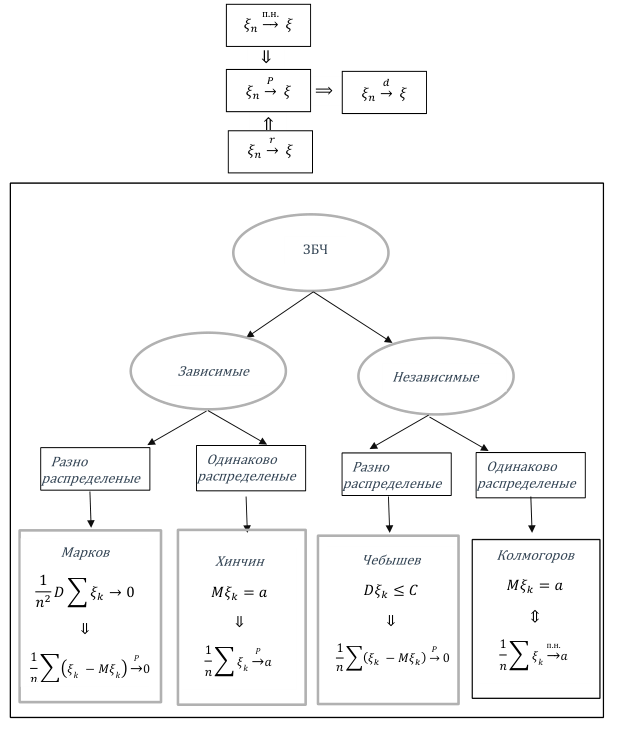
\includegraphics[width=0.8\textwidth]{Figures/resume.png}
	\label{fig:resume}
\end{figure}

  \chapter{Лекция 3 - 2023-09-20}
\section{Мотивация}
Пусть $ X = X_1, X_2, \ldots, X_n $ есть выборка (реализация случайной величины
$ \xi $, причём $ \{\xi_n\} $ независимы) из \textsl{известного}
распределения $ F(x, \theta) $, зависящего от \textsl{неизвестного} параметра $
\theta$.

\textsc{Задача}. Оценить значение параметра $ \theta $.

\begin{definition}
   Назовём функцию от выборки
	 \[
		 \widehat \Theta_n = f\left(x_1, x_2,\dots, x_n\right)
	 \]
	 \emph{оценкой параметра $\Theta$}, или \emph{статистикой}.
\end{definition}

Перечислим некоторые \textbf{свойства оценок}.
\begin{definition}
Оценку $ \widehat \Theta_n $ параметра назовём несмещённой, если 
\[
		\mathsf M \widehat \Theta_n = \theta.
\]
\end{definition}

%\begin{definition}
%  Оценка параметра $\widehat{D_n} = f(x_1, x_2, \dots, x_n)$.
%\end{definition}

\begin{definition}
  Оценка $\widehat{D_n}$ называется несмещенной, если $M[\widehat{D_n}]$.
\end{definition}

\[
  M f(\bar{x}) = \int\limits_{R_n} f(x_1, x_2, \dots, x_n) \prod\limits_{j=1}^{n} p_{x_i} (x_i) \, dx_1 dx_2 \dots dx_n.
\]

$$f(x_1, \dots, x_n) \toP 0, n \to \infty$$

Если $f(x_1, \dots, x_n) \toPN 0$, то $\hat{D_n}$ - силнльно состоятельная.

\begin{definition}
	Оценка $ \widehat \Theta_n $ называется \emph{асимптотически несмещённой},
	если  
	\[
		\mathsf M \widehat \Theta_n \to \theta \quad \text{при } n\to\infty.
	\]
\end{definition}

\begin{definition}
	Оценка $\widehat \Theta_n$ называется \emph{состоятельной}, если  
	\[
		\widehat \Theta_n \to \theta \quad \text{при } n\to\infty.
	\]
\end{definition}

\begin{definition}
Наконец, если  
\[
	\widehat \Theta_n \toPN \theta \quad \text{при } n\to\infty,
\]
то оценку $ \widehat \Theta_n $ называют \emph{сильно состоятельной}.
\end{definition}



%Пусть $x_1, \dots, x_n$ - выборка.
%$M X_i = a$.
%$$\hat{a_n} = ?$$

\section{Выборочное среднее}

\begin{definition}
	\emph{Выборочным средним} называют величину
	\[
		\hat a_n = \bar{X} = \frac{1}{n} \sum\limits_{i=1}^{n} x_i.
	\]
\end{definition}
Будем рассматривать $ \hat a_n $ как некоторую оценку математического ожидания
$ \mathsf M X_i = a $ рассматриваемой случайной величины. Обозначим кроме того
$ \mathsf D X_i = \sigma^2 $.

Перечислим \textbf{свойства выборочного среднего}.
\begin{enumerate}
	\item \textsc{Несмещённость}.
		\[
			M \bar{X} = M\left(\frac{1}{n} \sum\limits_{i=1}^{n} x_i\right) =
			\frac{na}{n} = a.
		\]
	\item \textsc{Сильная состоятельность}.
	\item \textsc{Дисперсия}. Дисперсия выборочного среднего стремится к нулю при увеличении $ n $.
		Действительно,  
		\[
			\mathsf D\bar X = \frac{1}{n^2} \sum_{i=1}^n \mathsf D X_i =
			\frac{\sigma^2}{n}.
		\]
		
\end{enumerate}

\section{Выборочная дисперсия (исправленная)}
\begin{definition} 
	\emph{Выборочной дисперсией} будем называть величину
\[ 
	S^2 = \frac{1}{n-1} \sum\limits_{i=1}^{n} \left( X_i-\bar{X}\right)^2.
\]
\end{definition}

Перечислим \textbf{свойства выборочной дисперсии}.
\begin{enumerate}
	\item Математическое ожидание выборочной дисперсии $ \mathsf M S^2 = \sigma^2
		$ равно истинной дисперсии. 
	\begin{multline*}
  \mathsf M S^2 = \frac{1}{n-1} \mathsf M\left[\sum_{i=1}^{n} \left(X_i - a - \left(\bar{X} - a\right)^2\right)^2 \right] = \\
  = \frac{1}{n-1} \sum \mathsf M (X_i-a)^2 - 2 \mathsf M\left[ \left(\bar{X} - a\right) \sum
	(X_i - a) \right] + \mathsf M (\bar{X} -a)^2 = \\
  = \frac{1}{n-1} \left[ n \sigma^2 - 2 n \mathsf M(\bar{X}-a)^2 + n \mathsf M (\bar{X}-a)^2 \right] = \\
  = \frac{1}{n-1} \left[ n \sigma^2 - n \frac{\sigma^2}{n} \right] = \sigma^2.
\end{multline*}
\item \textsc{Состоятельность}. 
\[
	S_n^2 = \frac{1}{n-1} \sum_{i=1}^n (X_i - \bar{X})^2 = \frac{n}{n-1} \left[
\frac{1}{n} \sum_{i=1}^n X_i^2 - \bar{X}^2 \right] \toPN \sigma^2 \quad
\text{при } n \to \infty.
\]
Действительно,
\[
	\frac{n}{n-1} \to 1, \qquad \bar X^2 \to a^2, 
\]
и, наконец,
\[
	\frac{1}{n} \sum_{i=1}^n X^2_i \toPN \sigma^2 + a^2
\]
в силу усиленного закона больших чисел.
\item \textsc{Дисперсия}.
\[
\mathsf D S^2 = \dfrac{\mu_4}{n} - \frac{\sigma^4 (n-3)}{n (n-1)} = O \left(\frac{1}{n}
\right),
\]
где $\mu_4 = \mathsf M X_i^4$ --- четвертый момент.
\end{enumerate}

\begin{theorem}[достаточное условие состоятельности]

Пусть $\widehat\Theta_n$ --- асимптотически несмешщенная оценка $\Theta$ и
$\mathsf D \bar\Theta_n \to 0$ при $ n \to \infty$.

Тогда $\widehat\Theta_n$ --- состоятельная оценка $\Theta$.
\end{theorem}
\begin{proof}
	Запишем условие состоятельности оценки $ \widehat\Theta_n $ в следующем виде:
\[
  | \widehat\Theta_n - \Theta| = |\widehat \Theta_n - \mathsf M \widehat\Theta_n
	+ \mathsf M \widehat\Theta_n
	- \Theta| \leqslant
	|\widehat\Theta_n - \mathsf M\widehat\Theta_n| + | \mathsf M\widehat\Theta_n -
	\Theta| \toP 0,
\]
где второе слагаемое стремится к нулю ввиду ассимптотической несмещённости $
\widehat\Theta_n $. Для сколь угодно малого $ \varepsilon > 0 $ имеем кроме того
\[
  P( | \widehat\Theta_n - \mathsf M \widehat\Theta_n| > \varepsilon) \leqslant
	\frac{|\widehat\Theta_n - \mathsf M
	\widehat\Theta_n| ^2} {\varepsilon^2} =  \frac{\mathsf D \widehat\Theta_n}
	{\varepsilon^2} \to 0 \quad \text{при } n \to\infty,
\]
что и доказывает утверждение.

\end{proof}



\section{Выборочная функция распределения}
\begin{definition}
	Назовём \emph{индикатором} функцию
\[
	I(x) = \begin{cases}1, &x>0,\\
	0, &x\leqslant 0.\end{cases}
\]
\end{definition}
Видно, что индикатор непрерывен слева.

\begin{definition}
	Назовём \emph{выборочной функцией распределения} функцию
	\[
		\widehat F_n (x) = \frac{1}{n} \sum_{i=1}^n I(x-X_i).
	\]
\end{definition}

\noindent Назовём некоторые из \textbf{свойств выборочной функции распределения}.
\begin{enumerate}
	\item \textsc{Несмещенность}.
\[
  \mathsf M \widehat F_n (x) = \mathsf M \frac{1}{n} \sum I(x-X_i)
\]

\item \textsc{Сильная состоятельность}.

\item \textsc{Теорема Гливенко -- Кантелли}.
	\begin{theorem}[Гливенко -- Кантелли] 

		\[
			\sup_x |\widehat F_n (x) - F(x)| \toPN 0.
		\]
	\end{theorem}
\begin{proof}
	б/д
	%TODO: (proof)

\end{proof}

\item \textsc{Неравенство Дворецкого -- Кифера -- Волфовица}.

\[
	P(\sup_x |\widehat F_n(x) - F(x)| > \varepsilon) \leqslant 2 e^{-2n
	\varepsilon^2}.
\]
\begin{proof}
	б/д
	%TODO: (proof)

\end{proof}
\begin{corollary*} 
	Возьмём для некоторого $ \alpha > 0 $
\[
		\varepsilon = \sqrt{ \frac{\ln 2/\alpha }{2n}}.
	\]
	Тогда
	\[
		P\left(\sup_x |\widehat F_n (x) - F(x)| \leqslant \varepsilon\right)
		\geqslant 1 - 2 e^{-2n \varepsilon^2} = 1-\alpha.
	\]
\end{corollary*}
Таким образом, с вероятностью $ 1 - \alpha $ имеем
\[
		\widehat F_n (x) - \varepsilon \leqslant F(x) \leqslant \widehat F_n(x) +
		\varepsilon,
\]
или более точно,
\begin{gather*}
	L(x) \leqslant F(x) \leqslant R(x), \quad \text{где}\\
		L(x) = \max \{ \widehat F_n(x) - \varepsilon,\, 0 \}, \qquad R(x) =
		\min \{ \widehat F_n(x) + \varepsilon, \,1 \}.
	\end{gather*}

\item \textsc{Общие свойства}:
	\begin{enumerate}
	\item Пределы  выборочной функции распределения при $ x \to \pm\infty $ равны
		соответственно
		\[
		\widehat F_n(+\infty) = 1, \qquad \widehat F_n(-\infty) = 0.
	\]
	\item Выборосная функция функция распределения $\widehat F_n(x)$ не убывает.
	\item Из первых двух свойств легко получаем 
	\[
			0 \leqslant \widehat F_n(x) \leqslant 1.
	\]
	
	\end{enumerate}
\end{enumerate}

\begin{theorem} Если выборка $x_1, \dots, x_n$ получена из закона распределения
	$F(x)$, то $\widehat F_n(x)$ есть дискретная случайная величина с распределением
\[
	P(\widehat F_n(x) = k/n) = C_n^k F(x)^k (1-F(x))^{n-k} 
\]
\end{theorem}
\begin{proof} 
	Из определения выборочной функции распределения
\[
	\widehat F_n \left(x\right) = \frac{1}{n} \sum_{i=1}^n I\left(x-X_i\right)
\]
сразу виден закон распределения Бернулли с вероятностью успеха $ p = F(x) $.

\end{proof}

\begin{corollary}
	\[
		\mathsf M \widehat F_n (x) = \frac{np}{n} = p = F(x).
	\]
\end{corollary}
\begin{corollary}
	\begin{multline*}
		\mathsf D \widehat F_n (x) = \frac{npq}{n^2} = \frac{F(x) (1 - F(x))}{n}
		\Leftrightarrow\\\Leftrightarrow
 \mathsf M (\widehat F_n(x) - F(x))^2 \to 0\Leftrightarrow\\
\Leftrightarrow \widehat F_n (x) \to F(x) \quad \text{(среднеквадратично при $
n\to\infty $)}.
\end{multline*}
\end{corollary}
\setcounter{corollary}{0}


\section{Порядковая статистика}
\begin{definition}
	Выборка, упорядоченная по возрастанию
	\[
		X_{(1)} \leqslant \dots \leqslant X_{(n)},
	\]
	 называется \emph{вариационным рядом}.
\end{definition}
\begin{definition}
	Член  вариационного ряда $ X_{(k)} $ называют \emph{$ k $-ой порядковой статистикой}.
\end{definition}

\begin{definition}
Назовём \emph{размахом выборки} число
\[
	\omega = X_{(n)} - X_{(1)}.
\]
\end{definition}

\begin{theorem}
	Если независимая выборка взята из генеральной совокупности с
функцией распределения $F(x)$, то функции распределения крайних членов
вариационного ряда и их совместная функция распределения имеют вид 
\begin{align*}
	\text{1. }F_{X_{(n)}}(x) &= [F(x)]^n,\\
	\text{2. }F_{X_{(1)}}(x) &= 1 - [1 - F(x)]^n,\\
	\text{3. }F_{X_{(1)}, X_{(n)}} (x, y) &= [F(y)]^n - [F(y)-F(x)]^n, \quad x < y.
\end{align*}
\end{theorem}
\begin{proof} Проведём доказательсто по всем пунктам.
	\begin{enumerate}
		\item Из независимости случайных величин и равенства $ X_{(n)} = \max\limits_i X_i $ вытекает соотношение
	\[
		F_{X_{(n)}}(x) = P \left( X_{(n)} < x \right) = P \left( \bigcap_{k=1}^n (X_k <
		x)\right) = \prod_{k=1}^n P(X_k < x) = [F(x)]^n.
	\]
\item Аналогично для $ X_{(1)} $ получим 
\[
	F_{X_{(1)}}(x) = 1 - P(X_{(1)} \geqslant x) = 1 - \prod_{k=1}^n P(X_k \geqslant
	x) = 1 - [1- F(x)]^n.
\]
\item В последнем случае 
\begin{multline*}
	F_{X_{(1)}, X_{(n)}}(x,y) = P(X_{(1)} < x, \, X_{(n)} < y) = \\ = P(X_{(n)} < y ) -
	P\left(X_{(1)} \geqslant x, \, X_{(n)} < y \right) = \\ =
	[F(y)]^n - P \left( \bigcap_{k=1}^n (x \leqslant X_k < y ) \right)  = \\ =
	[F(y)]^n - \prod_{k=1}^n P(x \leqslant X_k < y) = \\ =
	[F(y)]^n - [F(y) - F(x)]^n, \quad x < y.
\end{multline*}
\end{enumerate}
\end{proof}
\begin{corollary*}
	Если выборка взята из абсолютно непрерывного закона $F(x)$ с 
плотностью $p(x)$, то плотности распределения крайних членов вариационного ряда и их 
совместная плотность имеют вид 
\begin{align*}
	p_{X_{(n)}}(x) &= n[F(x)]^{n-1}p(x),\\
	p_{X_{(1)}}(x) &= n[1-F(x)]^{n-1}p(x),\\
	p_{X_{(1)}, X_{(n)}}(x, y) &= n(n-1)[F(y)-F(x)]^{n-2}p(x)p(y), \quad x < y.
\end{align*} %TODO: как получить последнее? (вписать формулу)
\end{corollary*}

\begin{theorem}
	Если независимая выборка взята из генеральной совокупности с
плотностью распределения $p(x)$, то плотность распределения $k$-ой порядковой
статистики имеет вид 
\[
	p_{X_{(k)}}(x) = n C^{k-1}_{n-1} \left[ F(x) \right]^{k-1} [1 - F(x)]^{n-k}
	p(x).
\]
\end{theorem}
\begin{proof}
	%TODO: поменять доказательство с инженерного на математическое (см. книгу
	%<<Порядковые статистики>>)
Зафиксируем $ x \in \mathbb R $ и выберем столь малое $ \Delta x $, что в
промежуток $ [x, x+ \Delta x) $ может попасть только один элемент выборки (закон
абсолютно непрерывный!). Тогда согласно полиномиальной схеме событие 
$(x \leqslant X_{(k)} < x + \Delta x)$ означает, что какие-то $ k - 1 $ элементов
выборки попали в промежуток $ (-\infty, x) $, 
один элемент в промежуток $[x, x + \Delta x)$, а остальные в $[x + \Delta x,
+\infty)$. Поскольку вероятности 
попаданий в эти множества равны $ F(x) $, $ p(x)\Delta x $ и $(1 - F(x + \Delta
x))$ соответственно, то  
\begin{multline*}
	F_{X_{(k)}}(x+\Delta x) - F_{X_{(k)}} (x) = P(x \leqslant X_{(k)} < x + \Delta
	x) = \\ =
	\frac{n!}{(k-1)!1!(n-k)!} [F(x)]^{k-1} p(x) \Delta x [1 - F(x + \Delta
	x)]^{n-k} = \\ =
	n C^{k-1}_{n-1} [F(x)]^{k-1} [1 - F(x + \Delta x)]^{n-k} p(x)\Delta x.
\end{multline*}
Завершим доказательство делением на $ \Delta x $ и переходом к пределу при $
\Delta x \to 0 $.

\end{proof}



\section{Примеры}
\begin{ex}
	Пусть дана выборка объёма $ n $ из показательного закона с параметром $ \alpha
	$. Тогда
	\[
		p_{X_{(1)}}(x) = n(1 - (1 - e^{-\alpha x}))^{n-1} \alpha e^{-\alpha
		x} = n \alpha e^{-n\alpha x}.
	\]
\end{ex}
\begin{ex}
	Найдём математическое ожидание и дисперсию $ X_{(k)} $, если выборка получена
	из равномерного распределения на $ [0, a] $. 

	Математическое ожидание минимального члена вариационного ряда равно
	\begin{multline*}
		\mathsf M X_{(1)} = \frac{n}{a }\int\limits_{0}^{a} x\cdot \left( 1 - \frac{x}{a}
		\right)^{n-1}\,dx \to \left[ \begin{aligned} u &= 1 - x/a \\ dx &= -a\,du
		\end{aligned}\right] \to an \int\limits_{0}^{1} \left( 1 - u \right) \cdot
		u^{n-1}\,du =\\=
		\frac{an}{n+1} \left. \left( 1 - \frac{x}{a} \right)^{n+1} \right|^a_0 - a
			\left.\left( 1 - \frac{x}{a} \right)^n \right|^a_0 = - \frac{an}{n+1} + a
				= \frac{a}{n+1}.
	\end{multline*}
	
	Математическое ожидание максимального члена вариационного ряда равно 
	\[
	\mathsf M X_{(n)} = \frac{n}{a}\int\limits_{0}^{a} x
	\left(\frac{x}{a}\right)^{n-1}\,dx = \frac{an}{n+1} \left.\left( \frac{x}{a}
	\right)^{n+1} \right|^a_0 = \frac{an}{n+1}.
	\]
	Отсюда видно, что $ X_{(n)} $ --- асимптотически несмещённая оценка параметра
	$ a $.

	Наконец, 
	\begin{multline*}
		\mathsf M X_{(k)} = \frac{n}{a}\int\limits_{0}^{a} x\cdot C^{k-1}_{n-1}
		\left(\frac{x}{a}\right)^{k-1} \left( 1 - \frac{x}{a} \right)^{n-k}\,dx = \\
		= an C^{k-1}_{n-1} \int\limits_{0}^{1}
		u^k(1-u)^{n-k}\,du = 
		an C^{k-1}_{n-1} B(k+1, n-k+1)  = \\ = a \frac{(n-1)!n}{(k-1)! (n-k)!}
		\frac{\Gamma(k+1) \Gamma(n-k+1)}{\Gamma(n+2)} = \frac{ak}{n+1},
	\end{multline*}
	где $ u = x/a $.
\end{ex}

  \chapter{Лекция 4 - 2023-09-27 - Методы получения точечных оценок: моментов, максимального
правдоподобия. Свойства точечных оценок.}

\section{Вероятности для вариационного ряда}

\begin{theorem}
  $X_1, X_2, \dots, X_n$ - независимыя выборка из з.р. $F(X)$

  тогда $F_{X_{(n)}} = (F(x))^n$, $F_{X_{(1)}} = 1 - (1-F(x))^n$.

  если имеется плотность $p(x)$, то $p_{X_{(n)}} = n (F(x))^{n-1} p(x)$, $p_{X_{(1)}} = n (1-F(x))^{n-1} p(x)$, $p_{X_{(1)}, X_{(n)}} = n (n-1) (F(y) - F(x))^{n-2} p(x) p(y)$.
\end{theorem}

\begin{proof}
  \begin{multline}
    F_{X_{(n)}} = P(X_{(n)} < x) = P\left(\bigcap_{k=1}^n (X_k < x)\right) = \prod_{k=1}^n P(X_k < x) = (F(x))^n\\
    F_{X_{(1)}} (x) = P(X_{(1)} < x) = 1 - P(X_{(1)} \geqslant x) = \dots = 1 - (1-F(x+0))^n = 1 - (1-F(x))^n \\
    F_{X_{(1)}, X_{(n)}} (x, y) = P(X_{(1)} < x, X_{(n)} < y) = P(X_{(n)} < y) - P(X_{(n)}, X_{(1)} \geqslant x) = \\
    F_{X_{(n)}} (y) - P(\bigcap_{k=1}^n (x \leqslant X_k < y)) = (F(y))^n - (F(y) - F(x))^n
    % \\
    % TODO: доказательство PX(1) X(n) (x, y)
  \end{multline}
\end{proof}

\begin{ex}
  $X_1, X_2, \dots, X_n ~ E(\alpha)$
  $F_{x_i} (x) = 1- e^{-\alpha x}, x\geqslant 0.$
  $F_{X_{(1)}} (x) = 1 - (1-1+e^{-\alpha x})^n = 1 - e^{-\alpha x} \Rightarrow X_{(1)} \sim E(n\alpha)$
\end{ex}

\begin{theorem}
  $X_1, X_2, \dots, X_n$ - независимая выборка из з.р. с плотностью $p(x)$.
  тогда $p_{X_{(k)}} = n C_{n-1}^{k-1} (F(x))^{k-1} (1-F(x))^{n-k} p(x)$.
\end{theorem}

\begin{proof}
  \[
    P(x\leqslant X_{(k)} < x+\Delta x) = \dfrac{n!}{(k-1)! (n-k)!} (F(x))^{k-1} p(x) \Delta x (1-F(x+\Delta x))^{n-k}
  \]
\end{proof}

\section{Методы построения точечных оценок параметров}

$X_1, X_2, \dots, X_n \sim F(x, \theta_1, \theta_2, \dots, \theta_n)$

\subsection{Метод моментов}

$\hat{\mu}_k = \frac{1}{n} \sum X_i^k$ - эмпирический момент k-го порядка.

$\mu_k = \int\limits_{-\infty}^{+\infty} x^k dF(x, \bar{\theta})$

По закону больших чисел: $\hat{\mu}_k \toPN \mu_k$

\[
\begin{cases}
  \hat{\mu}_1 = \mu_1(x, \bar{\theta}), \\
  \hat{\mu}_2 = \mu_2(x, \bar{\theta}), \\
  \dots = \dots \\
  \hat{\mu}_r = \mu_r(x, \bar{\theta})
\end{cases}
\]

\begin{ex}
  Пусть $X_1, \dots, X_n \sim E(\alpha)$.

  Тогда $\hat \mu_1 = \bar{X} = \frac{1}{\alpha} = \mu_1 \Rightarrow \alpha = \frac{1}{\bar{X}}$ - несмещённая.
  \begin{proof}
    $X_k \sim \alpha e^{-\alpha x} \equiv \gamma_{\alpha, 1}$
    Тогда $\xi = \sum X_k \sim \gamma_{\alpha, n}$.
    $M \hat \alpha_n = M \frac{n}{\xi} = \int\limits_0^{+\infty} \frac{n}{x} \dfrac{\alpha^n x^{n-1} e^{-\alpha x}}{\Gamma(n)} \, dx = \frac{n \alpha}{\Gamma(n)} \int\limits_0^{+\infty} (\alpha x)^{n-2} e^{-\alpha x} \, dx = \dfrac{n\alpha \Gamma(n-1}{\Gamma(n)} = \dfrac{n\alpha}{n-1} \to \alpha$
  \end{proof}
\end{ex}

\subsection{Оценки максимального правдоподобия}

$X_1, X_2, \dots, X_n \sim p(x, \bar\theta) \text{или} P(\xi = X_k)$

\begin{definition}
  $\mathcal{L} (X_1, X_2, \dots, X_n, \hat\theta) = $
  В случае непрерывной величины: $\mathcal{L} = \prod_{k=1}^n P(X_k, \hat \theta)$
  В случае дискретной: $\mathcal{L} = P(\xi_1 = X_1, \xi_2 = X_2, \dots, \xi_n = X_n) = \prod P(\xi_k = X_k)$

  $\mathcal{L}$ исследуется на максимум по параметру $\theta$.
\end{definition}

$\dfrac{\partial \mathcal{L}}{\partial \theta} = 0 \Leftrightarrow \frac{1}{\mathcal{L}} \dfrac{\ln \mathcal{L}}{\partial \theta} = 0$

\begin{ex}
  $X_1, X_2, \dots, X_n \sim Pois(\lambda)$
  $P(\xi=x_k) = \dfrac{\lambda^{X_k}}{(X_k)!} e^{-\lambda}$

  $\mathcal{L}(X_1, \dots, X_n, \lambda) = \prod \dfrac{\lambda^{X_k}}{(X_k)!} e^{-\lambda}$

  $\ln \mathcal{L} = \sum X_k \ln\lambda - n \lambda - \ln \prod (X_k)!$

  $\dfrac{\partial \ln \mathcal{L}}{\partial \lambda} = \dfrac{\sum X-k}{\lambda} - n = 0 \Rightarrow \bar{\lambda_n} = \frac{1}{n} \sum X_k$
\end{ex}

\begin{ex}
  $X_1, X_2, \dots, X_n \sim E(\alpha)$

  $\mathcal{L}(X_1, \dots, X_n, \alpha) = \prod \alpha e^{-\alpha x_k} = \alpha^n e^{-\alpha \sum x_k}$

  $\ln \mathcal{L} = n \ln\alpha - \alpha \sum x_k$

  $\dfrac{\partial \ln\mathcal{L}}{\partial \alpha} = \frac{n}{\alpha} - \sum x_k$
\end{ex}

\subsection{Сравнение оценок}

\begin{definition}
  Если $\hat \theta_n$ и $\widehat{\widehat{\theta}}_n$ - две несмещенные оценки параметра $\theta$.
  Если $D \hat\theta_n < D \hat\hat\theta_n$, то говорят, что $\hat\theta_n$ - более эффективна, чем $\hat\hat\theta_n$
\end{definition}

\begin{ex}
  $X_1, X_2, \dots, X_n \sim R[\theta-\frac{1}{2}, \theta+\frac{1}{2}]$

  $\hat\theta_n = \frac{1}{2} (X_{(1)} + X_{(n)})$
  
  $\Hat{\Hat{\theta}}_n = \bar X$

  $D\hat\theta_n = \dots = \dfrac{1}{8 (n+1) (n+2)} \sim \dfrac{c}{n^2}$

  $D\Hat{\Hat{\theta}}_n = \dfrac{1}{12n}$
\end{ex}

\begin{theorem}[Неравенство Рао-Крамера]
  Если $X_1, X_2, \dots, X_n$ - выборка из закона распределения с плотностью $p(x, \theta)$ и $\int\limits_R p(x, \theta) \, dx = 1$ допускает дифференцирование по $\theta$.
  Тогда $\forall$ несмещенной оценки $\hat\theta_n$ имеет место:
  $$D\hat\theta_n \geqslant \frac{1}{I_n(\theta)} = \frac{1}{n I_1(\theta)},$$
  где $I_n(\theta) = M\left( \dfrac{\partial \ln \mathcal{L}}{\partial \theta} \right)^2$ - информация Фишера,
    $I_1(\theta) = M\left( \dfrac{\partial\ln p(x, \theta)}{\partial\theta} \right)^2$
\end{theorem}

\begin{proof}
  $1 = \int\limits_{R^n} p(x, \theta) \, dx \Rightarrow 0 = \int\limits_{R^n} \dfrac{\partial p(x, \theta)}{\partial\theta} \, dx = \int\limits_{R^n} \dfrac{\ln p(x, \theta)}{\partial\theta} p(x, \theta) \, dx$

  $\hat\theta_n = \phi(X_1, X_2, \dots, X_n), \theta = \int_{R^n} \phi(x) p(x, \theta) \, dx \Rightarrow 1 = \int_{R^n} \phi(x) \dfrac{\partial \ln p(x, \theta)}{\partial\theta} p(x, \theta) \, dx$

  $\Rightarrow 1 = \int_{R^n} (\phi(x)-\theta) \dfrac{\partial \ln p(x, \theta)}{\partial \theta} p(x, \theta) \, dx$

  $1 \leqslant \int_{R^n} (\phi(x) - \theta)^2 p(x, \theta) \, dx \cdot \int_{R^n} (\dfrac{\partial\ln p(x, \theta)}{\partial\theta})^2 p(x, \theta) \, dx$

  $I_n(\theta) = M \left(\dfrac{\partial\ln L(X_1, X_2, \dots, X_n, \theta)}{\partial\theta}\right)^2 = D \dfrac{\partial \ln L}{\partial\theta} = \sum D\dfrac{\partial \ln p(x_k, \theta)}{\partial\theta} = n I_1(\theta)$

  $\ln L(X, \theta) = \sum \ln p(x_k, \theta)$
\end{proof}

\begin{ex}
  $X_1, \dots, X_n \sim R[\theta-1/2, \theta+1/2]$

  $p(x, \theta) = I(\theta-1/2 \leqslant x \leqslant \theta+1/2)$

  $1 = \int\limits_{-\infty}^{+\infty} I \, dx$ - не допускает дифференцирование по параметру.
\end{ex}

\begin{ex}
  $X_1, X_2, \dots, X_n \sim E(\alpha)$

  $p(x, \alpha) = \alpha e^{-\alpha x}$

  $I_1(\alpha) = M (\dfrac{\partial\ln p(X_1, \alpha)}{\partial\alpha})^2$

  $\ln p(X_1, \alpha) = \ln \alpha - \alpha X_1$

  $\dfrac{\partial \ln p}{\partial\alpha} = \frac{1}{\alpha} - X_1$

  $I_1(\alpha) = M (\frac{1}{\alpha} - X_1)^2 = D X_1 = \dfrac{1}{\alpha^2}$
\end{ex}

Вывод: $\forall$ несмещенной оценки $\hat\alpha_n$: $D \hat\alpha_n \geqslant \dfrac{1}{n \frac{1}{\alpha^2}} = \frac{\alpha^2}{n}$ 


  \chapter{Лекция 5 - 2023-10-04 - Достаточные статистики. Критерий факторизации}
\section{Достаточные статистики}
Пусть $ X_1, X_2, \ldots, X_n $ --- выборка из распределения, зависящего от
параметра $ \bar \theta $ (реализация случайного вектора $ \bar \xi = (\xi_1,
\xi_2, \ldots, \xi_n) $ с независимыми компонентами).

\begin{definition}
  Вектор-функция $\bar t = \bar t(X_1, X_2, \dots, X_n)$ называется \emph{достаточной
	статистикой} для оценки параметра $\bar{\theta}$, если условная функция
	распределения
	\[
		F_{\bar \xi} (X_1, X_2, \dots, X_n\, | \,\bar{t} (\xi_1, \dots, \xi_n)
		= \bar t)
	\]
	не зависит от $\bar\theta$ при любых значениях $\bar t$. 
\end{definition}

\begin{remark*}
Статистика $ \bar t $ является достаточной для оценки параметра $ \theta $, если
\begin{enumerate}
	\item \textsc{Дискретный случай}. Условные вероятности 
	\[
			P(\xi_1 = X_1, \xi_2 = X_2, \ldots, \xi_n = X_n\, \mid \, \bar t(\bar \xi) = \bar
			t)
	\]
	не зависят от $ \theta $ при любых значениях $ \bar t $.
\item \textsc{Непрерывный случай}. Условные плотности  
\[
	p_{\bar \xi} (X_1, X_2, \ldots, X_n\, |\,\bar t(\bar \xi) = \bar t)
\]
не зависят от $ \theta $ при любых значениях $ \bar t $.
\end{enumerate}

\end{remark*}

\begin{ex}
  Пусть $X_1, X_2, \dots, X_n$ распределены по Бернулли с вероятностью успеха $p$
	(последовательность 0 и 1).

	Докажем, что статистика $\sum_{k=1}^n X_k$ достаточна для оценки параметра $p$.
Найдём условные вероятности
  \begin{multline*}
		P\left(\xi_1 = X_1, \dots, \xi_n = X_n\,\Big|\, \sum_{k=1}^n \xi_k =
		t\right) = \\
		= \frac{P(\xi_1 = X_1, \dots \xi_n = X_n, \sum \xi_k = t)}{P\left(\sum_{k=1}^n \xi_k = t\right)} = \\
    = \begin{cases}
			p = 0, &t \neq \sum_{k=1}^n X_k, \\
			\frac{ p^t (1-p)^{n-t} }{ C_n^t p^t (1-p)^{n-t} } = \frac{1}{C_n^t}, &t
			= \sum_{k=1}^n X_k.
    \end{cases}
  \end{multline*}
	Действительно, знаменатель по теореме Бернулли равен $ C^t_n p^t(1-p)^{n-1} $.
	Числитель равен нулю, если $ t \ne \sum_{k=1}^n $ и $ p^t(1-p)^{n-t} $ в ином
	случае.

	Таким образом, условная вероятность в любом случае не зависит от $ p $.
\end{ex}

\begin{theorem}[критерий факторизации]
  Если $X_1, X_2, \dots, X_n \sim F(x, \bar\theta)$, то $\bar t = \bar t (X_1,
	\dots, X_n)$ является достаточной статистикой для оценки $\bar\theta$ тогда и
	только тогда, когда 
  \[
    \mathscr{L}(X_1, X_2, \dots, X_n, \bar\theta) = h(X_1, \dots, X_n)
		g(\bar\theta, \bar t (X_1, X_2, \dots, X_n)),
  \]
  где $h$ не зависит от $\theta$, $g$ не зависит от $X_1, X_2, \dots, X_n$
	(разве что через $\bar t$)
\end{theorem}

\begin{proof}
	Проведём доказательство в обе стороны.
	\begin{enumerate}
		\item $\boxed{\Leftarrow}$ Пусть
			\[
				\mathscr L(X_1, X_2, \ldots, X_n, \theta) = g\left(\bar \theta, \bar t(X_1,
				X_2, \ldots, X_n) \right)h(X_1, \ldots, X_n).
			\]

			Имеем
  \begin{multline*}
    P(\xi_1 = X_1, \dots, \xi_n = X_n \, | \, \bar t (\xi_1, \dots, \xi_n) = \bar t)
    = \\ = \frac{P(\xi_1=X_1, \dots, \xi_n = X_n, \bar t(X_1, \dots, X_n) = \bar
		t_0)}{P(\bar t(\xi_1, \dots, \xi_n) = \bar t_0)}.
  \end{multline*}
При $ \bar t(X_1, X_2, \ldots, X_n) \neq \bar t_0$ полученное выражение,
очевидно, равно нулю. Рассмотрим случай $ \bar t(X_1, X_2, \ldots, X_n) = \bar
t_0 $. Тогда числитель будет равен функции правдоподобия $ \mathscr L(X_1,
\ldots , X_n, \bar \theta) $, а знаменатель 
\[
		P(\bar t(\xi_1, \ldots, \xi_n) = \bar t) = \sum_{\bar Z \colon \bar t(\bar
		Z) = \bar t_0} P(\xi_1 = Z_1, \ldots, \xi_n = Z_n) = \sum_{\bar Z\colon \bar
		t(\bar Z) = \bar t_0}\mathscr L(Z_1, \ldots, Z_n, \bar \theta). 
\]

Следовательно, для рассматриваемого случая имеем
\begin{multline*}
    P(\xi_1 = X_1, \dots, \xi_n = X_n \, | \, \bar t (\xi_1, \dots, \xi_n) =\\=
		\frac{P(\xi_1 = X_1, \ldots, \xi_n = X_n)}{\sum P(\xi_1 = Z_1, \ldots, \xi_n = Z_n)} =\\= \frac{h(X_1, \dots, X_n)
		g(\bar \theta, \bar t(X_1, \dots, X_n))}{\sum h(Z_1, \dots, Z_n)
		g(\bar\theta, \bar t(Z_1, \dots, Z_n)} = \frac{h(X_1, \dots, X_n)}{\sum h(Z_1,
		\dots, Z_n)},
\end{multline*}
где суммирование, как и прежде, производится по таким $ \bar Z $, что $ \bar
t(\bar Z) = \bar t_0 $. Результат не зависит от $ \bar \theta $, что и
требовалось доказать.
\item $\boxed{\Rightarrow}$
  Докажем, обратно, что если вероятность
	\[
		P(\xi_1 = X_1, \dots, \xi_n = X_n \,| \,\bar
		t(\xi_1, \dots, \xi_n)
		= \bar t)
	\]
	не зависит от $\bar \theta$, то $\mathscr{L}$ факторизуется. Действительно, в
	случае $ \bar t_0 = \bar t(X_1, \ldots, X_n) $
  \begin{multline*}
    \mathscr{L} (X_1, \dots, X_n, \bar\theta) = P_{\bar\theta} (\xi_1 = X_1,
		\dots, \xi_n = X_n) =\\= P_{\bar\theta} (\xi_1 = X_1, \dots, \xi_n = X_n \,
		|\, \bar
		t(\bar\xi) = \bar t) \cdot P(\bar t(\bar\xi) = \bar t).
  \end{multline*}
  Первый множитель не зависит от $\bar\theta$, второй зависит от $X_1, \dots,
	X_n$ только через $\bar t(X_1, \dots, X_n)$.

\end{proof}

\begin{remark}
  \begin{align*}
		\mathscr{L} &= h(X_1, \dots, X_n) g(\bar\theta, \bar t(X_1, \dots, X_n),\\
		\ln \mathscr{L} &= \ln h + \ln g,\\
		\frac{\partial \ln g}{\partial \bar \theta} &= \frac{\partial \ln \mathscr{L} (\bar\theta, \bar t(X_1, \dots,
	X_n))}{\partial \bar\theta}.
  \end{align*}
  $\Rightarrow$ ОМП функция от $\bar t(X_1, \dots, X_n)$
  % что значит последняя строка?
  % TODO не понял о чём это замечание, скорее всего ошибка
\end{remark}

\begin{ex}
	Пусть $X_1, \dots X_n \sim \operatorname{Pois}(\lambda)$, 
  \[
    P(X_1, \dots, X_n, \lambda) = P_\lambda (\xi_1=X_1, \dots, \xi_n=X_n) =
		\prod_{k=1}^n P(\xi_k = X_k) = \prod_{k=1}^n \frac{\lambda^{X_k}}{(X_k)!}
		e^{-\lambda} =
		\frac{\lambda^{\sum X_k}}{\prod_{k=1}^n (X_k)!}  e^{-n\lambda},
  \]
	а значит, $\sum_{k=1}^n X_k$ --- достаточная статистика для оценки $\lambda$
	(как и $\bar X$).
\end{ex}

\begin{ex}
  Пусть $X_1, \dots, X_n \sim N(a, \sigma)$.
  \begin{multline*}
		\mathscr{L} (X_1, \dots, X_n, a, \sigma) = \prod_{k=1}^n \frac{1}{\sqrt{2\pi}
		\sigma} \exp\left(-\frac{(X_k-a)^2}{2\sigma^2}\right) =\\= 
		\left(\frac{1}{\sqrt{2\pi}\sigma} \right)^n
		\exp\left(-\frac{1}{2\sigma^2} \sum_{k=1}^n (X_k-a)^2\right) = \\ =
		\left(\frac{1}{\sqrt{2\pi}\sigma}\right)^n \exp\left(-\frac{1}{2\sigma^2}
			\left(\sum_{k=1}^n
		X_k^2 - 2a \sum_{k=1}^n X_k + na^2\right)\right).
  \end{multline*}
  Здесь достаточной статистикой для $ (a, \sigma) $ будет $(\sum X_k^2, \sum
	X_k)$.

  В то же время
	\[
		\sum_{k=1}^n (X_k-a)^2 = \sum_{k=1}^n (X_k - \bar X + \bar X - a)^2 =
		\sum_{k=1}^n (X_k-\bar X)^2 + (\bar X - a)^2 n,
	\]
	поэтому пара
	\[
		\left(\bar X,\, S^2 = \frac{1}{n-1} \sum_{k=1}^n (X_k-\bar X)^2\right)
	\]
	является достаточной статистикой для $\sigma$ при известном $a$.
\end{ex}

\begin{ex}
	Пусть $X_1, \dots, X_n \sim \operatorname{Par}(\alpha, \theta)$. Плотность
	равна
	\[
		p(x, \theta, \alpha) = \frac{\alpha}{\theta}
		\left(\frac{\theta}{x}\right)^{\alpha+1}, \quad x\geqslant 0.
	\]

	Найдём функцию правдоподобия и вычленим достаточную статистику:
  \[
		\mathscr{L} (X_1, \dots, X_n, \alpha, \theta) = \prod_{k=1}^n \frac{\alpha}{\theta}
		\left(\frac{\theta}{x}\right)^{\alpha+1} I(X_k \geqslant 0) = \frac{\alpha^n
		\theta^{\alpha n}}{(\prod X_k)^{\alpha+1}} I(X_{(1)}\geqslant 0) \cdot 1.
  \]
Следовательно, 
  $(X_{(1)}, \prod X_k)$ --- достаточная статистика для закона Паретто.
\end{ex}

\section{Интервальные оценки (доверительные интервалы)}
Пусть $X_1, \dots, X_n$ --- выборка из распределения с плотностью $p(x,
\theta)$, а $1-\alpha$ --- \emph{уровень доверия}.

\begin{definition}
	\emph{Доверительным интервалом} для одномерного параметра $\theta$ с 
доверительной вероятностью $1  - \alpha$ называется любой интервал $(\theta_1, \theta_2)$, 
содержащий истинное значение параметра с вероятностью $1 - \alpha$.  
\end{definition}


\subsection{Принцип построения доверительных интервалов}
\begin{enumerate}
  \item Находим статистику $\eta = \varphi(X_1, \dots, X_n, \theta)$, закон
		распределения  которой $F_\eta (x)$ известен точно или приближенно и не
		зависит от $\theta$.
  \item Находим квантили $t_{\alpha/2}$ и $t_{1-\alpha/2}$, при этом
    \[ 
			F_\eta(t_{\alpha/2})  = \alpha/2,\quad F_\eta(t_{1-\alpha/2}) = 1 -
			\alpha/2.
		\]
		Тогда
    \[
      P(t_{\alpha/2} < \varphi(X_1, \dots, X_n, \theta) < t_{1-{\alpha/2}}) =
			F_\eta (t_{1 - \alpha/2}) - F_\eta (t_{\alpha/2}) = 1- \alpha
    \]
  \item Неравенство  
  \[
		t_{\alpha/2} < \varphi(X_1, \ldots, X_n, \theta) < t_{1-\alpha/2}
  \]
		разрешается относительно $\theta$: 
		\[
			\ubar \varphi(X_1, \ldots, X_n, \alpha) < \theta < \bar\varphi(X_1,
			\ldots, X_n, \alpha).
		\]
		Обозначив $ \theta_1 = \ubar\varphi(X_1, \ldots, X_n, \alpha) $, $ \theta_2
		= \bar\varphi(X_1, \ldots, X_n, \alpha)$, получаем доверительный интервал
		уровня $ 1 - \alpha $.
\end{enumerate}

\begin{ex}[для неизвестного $ a $ при известном $ \sigma $]
  Пусть $X_1, \dots, X_n \sim N(a, \sigma_0)$, где $\sigma_0$ известна.

  Тогда по методу моментов $\hat a = \bar X$. Отсюда
  \[
		\bar X = \frac{1}{n} \sum_{k=1}^n X_k \sim N\left(a,
		\frac{\sigma_0}{\sqrt{n}}\right).
  \]

	Следовательно, распределение
	\[
		\frac{\bar X - a}{\sigma_0} \sqrt{n} \sim N(0, 1)
	\]
не зависит от параметра $a$.

Получили
  \[
		-u_{1-\alpha/2} = u_{\alpha/2} &< \frac{\bar X - a}{\sigma_0} \sqrt{n} <
		u_{1-\alpha/2}, 
	\]
	или
	\[
		\bar X - \frac{u_{1-\alpha/2}}{\sqrt{n}} &< a < \bar X +
		\frac{u_{1-\alpha/2}}{\sqrt{n}}.
	\]
 \end{ex}

 \begin{ex}[для неизвестного $ \sigma $ при известном $ a $]
  Рассмотрим противоположный случай. Пусть $X_1, \dots, X_n \sim N(a_0,
	\sigma)$,
	и параметр $a_0$ известен.

	В этом случае
	\[
		\mathscr{L} (X_1, \dots, X_n, \sigma) = \prod_{k=1}^n \frac{1}{\sqrt{2\pi}
		\sigma} \exp\left(-\frac{(X_k - a)^2}{2\sigma^2}\right) =
		\left(\frac{1}{\sqrt{2\pi}\sigma}\right)^n \exp\left(-\frac{1}{2\sigma^2}
		\sum_{k=1}^n (X_k-a)^2\right).
	\]
	Следовательно, $\sum_{k=1}^n (X_k-a)^2$ (вместе с $ S_0^2 = 1/n \sum_{k=1}^n(X_k - a_0)^2 $) будет достаточной статистикой.

	При этом, как легко заметить,
	\[
		\sum\limits_{k=1}^n \frac{(X_k-a)^2}{\sigma^2} = \frac{S^2_0 n}{\sigma^2}
		\sim \chi^2 (n).
	\]

	Найдём квантили и разрешим неравенство:
  \begin{gather*} 
		\chi^2_{\alpha/2} (n) < \sum_{k=1}^n \frac{(X_k - a_0)^2}{\sigma^2} <
		\chi^2_{1 - \alpha/2} (n), \\
		\frac{\sum_{k=1}^n (X_k-a_0)^2}{\chi^2_{1 - \alpha/2} (n)} < \sigma^2 <
		\frac{\sum_{k=1}^n (X_k - a_0)^2}{\chi^2_{\alpha/2}(n)}.
  \end{gather*}
\end{ex}

\begin{ex}
  Произведено $n=36$ измерений, $\bar X = 9.3 \text{кОм},  \sigma_0 = 2
	\text{кОм}$. Найти доверительный интервал $1- \alpha = 0.95$ для оценки
	параметра $a$.

\[
  0.95 = P\left(\bar X - \frac{u_{0.975} \cdot 2}{\sqrt{36}} < a < \bar X + \frac{u_{0.975} \cdot 2}{\sqrt{36}}\right) \Leftrightarrow a \in (8.65, 9.95)
\]
\end{ex}

\begin{ex}[на показательный закон]
	Пусть
  $X_1, \dots, X_n \sim E(\lambda)$.
  Достаточной статистикой  будет $\hat \lambda = \frac{1}{\bar X}$. Докажем
	сначала, что
  \[
		2\lambda \sum_{k=1}^n X_k \sim \chi^2(2n).
	\]

	Действительно, имеем
	\[
		X_k \sim \lambda e^{-\lambda x} \Rightarrow \eta = 2\lambda X_k \sim \frac{1}{2}
		e^{-\frac{x}{2}} \equiv \chi^2 (2).
	\]

	Найдём квантили и разрешим неравенство: 
	\begin{gather*}
		\chi^2_{\alpha/2}(2n) < 2\lambda\sum_{k=1}^n X_k <
		\chi^2_{1-\alpha/2}(2n),\\
	\frac{\chi^2_{\alpha/2}(2n)}{2 n\bar X } < \lambda <
	\frac{\chi^2_{1-\alpha/2}(2n)}{2 n \bar X}.
	\end{gather*}
\end{ex}

\subsection{Приближенные доверительные интервалы}
  Пусть $X_1, \dots, X_n \sim F(x, \theta), \M_\theta X_i = a(\theta), \D_\theta
	X_i = d(\theta)$, и $n$ велико. 

	Тогда согласно центральной предельной теореме статистика
\[
	\frac{\sum_{i=1}^n X_i - n a(\theta)}{\sqrt{n d(\theta)}} \approx N(0, 1)
\]
в пределе распределена по стандартному нормальному закону, что даёт приближённое
равенство
\[
	P\left(u_{1 - \alpha/2} < \frac{\sum_{i=1}^n X_i - n a(\theta)}{\sqrt{n d(\theta)}}<
	u_{1-\alpha/2}\right) \approx 1 - \alpha.
\]

\begin{ex}[на биномиальный закон, $ k $ известно]
  Пусть $X_1, \dots, X_n \sim B(k, p)$, но $k$ известно, а $ p $ неизвестно.

	Известно, что 
	\[
		\M X_k = kp, \quad \D X_k = k p (1-p).
	\]
В этом случае
\[
	\frac{\sum_{k=1}^n X_k - n k p}{\sqrt{nkp(1-p)}} \in (-u_{1-\alpha/2}, u_{1-\alpha/2})
\]
с вероятностью, стремящейся к $ 1 - \alpha $. Чтобы не решать квадратные
неравенства, заменим ещё $ p $ под корнем в
знаменателе оценкой $\hat p = \frac{\bar X}{k}$ (потеря точности невелика). 

Найдём квантили и разрешим неравенство:
\begin{gather*}
	-u_{1-\alpha/2}\cdot \sqrt{nk \frac{\bar X}{k} \left(1 - \frac{\bar X}{k}\right)} <
	\sum_{k=1}^n X_k -
	nkp < u_{1-\alpha/2} \cdot \sqrt{nk \frac{\bar X}{k} \left(1 - \frac{\bar X}{k}\right)}, \\
	\frac{\bar X}{k} - \frac{u_{1-\alpha/2}\cdot \sqrt{\frac{\bar X}{k} \left(1 - \frac{\bar
	X}{k}\right)}}{\sqrt{nk}} < p < \frac{\bar X}{k} + \frac{u_{1-\alpha/2}
\cdot \sqrt{\frac{\bar X}{k} \left(1 - \frac{\bar X}{k}\right)}}{\sqrt{nk}}.
\end{gather*}
\end{ex}

  \chapter{Лекция 6 - 2023-10-11}

\section{Доверительные интервалы для параметров нормального закона}

$X_1, \dots, X_n \sim N(a, \sigma)$

\begin{theorem}
  Если $X_1, \dots, X_n \sim N(a, \sigma)$, то статистика $\bar X$ и $\dfrac{(n-1) S^2}{\sigma^2} = \dfrac{1}{\sigma^2} \sum\limits_{k=1}^n (X_k-\bar X)^2$ независимы и $\bar X \sim N(a, \dfrac{\sigma}{\sqrt{n}}$, $\dfrac{(n-1) S^2}{\sigma^2} \sim \chi^2(n-1)$
\end{theorem}

\begin{theorem}[Лемма]
  $n = 1, \eta = a \xi, p_\eta(y) = \dfrac{1}{|a|} p_\xi(y/a)$.
  Если $p_{\bar \xi} (\bar x)$ - плотность СВ $\bar\xi$, СВ $\bar\eta = A\xi$, $\exists A^{-1}$
  $p_{\bar\eta} (\bar y) = |det A|^{-1} p_{\bar\xi} (A^{-1} \bar y)$
\end{theorem}
\begin{proof}
  $$p(\bar\xi \in B) = p(A\xi \in AB) = p(\eta \in AB)$$
  $$ p(\xi \in B) = \int_B p_\xi (\bar x) \, d\bar x
  = \left|\, \begin{aligned}
    \bar x &= A^{-1} \bar y \\
    \bar y &= A \bar x \\
    d\bar x &= |det(A^{-1})| d\bar y
  \end{aligned} \,\right| 
  = \int_{AB} p_\xi(A^{-1} \bar y) |det A_{-1}| d\bar y 
  \Rightarrow p_{\bar \eta} (\bar y)
  = p_{\bar\xi} (A^{-1} \bar y) |det A^{-1}|$$
\end{proof}


\begin{proof}[доказательство первой теоремы]
  $X_1, \dots, X_n \rightarrow X_1', \dots, X_n'$
  $$\bar X' = \dfrac{1}{n} \sum\limits_{k=1}^n X_k' = \dfrac{1}{n} \sum \dfrac{(X_k - a)}{\sigma} = \dfrac{\bar X - a}{\sigma}$$
  $$\vec{X}' = (X_1', \dots, X_n')^T$$
  $$p_{\bar X'} (x) = \dfrac{1}{(\sqrt{2\pi})^n} e^{-\dfrac{1}{2} \bar x^T \bar x}$$
  $$\bar Y = C \bar X', C - \text{ортог}$$
  $$Y_1 = \dfrac{1}{\sqrt{n}} \sum X_k' = \sqrt{n} \bar X' = \dfrac{\bar X - a}{\sigma} \sqrt{n}$$
  $$Y_1^2 = n (\bar X')^2$$
  $$p_{\bar Y} (y) = |det C|^{-1} p_{\bar X} (C^{-1} \bar y) = \dfrac{1}{(\sqrt{2\pi})^n} e^{-\dfrac{1}{2} (C^{-1} \bar y)^T C^{-1} \bar y} = \dfrac{1}{(\sqrt{2\pi})^2} e^{-\dfrac{1}{2} \bar y^T \bar y}$$
  
  \begin{multline*}
    ? \bar X и \dfrac{(n-1) S^2}{\sigma^2}; \\
    \dfrac{(n-1) S^2}{\sigma^2} \dfrac{1}{\sigma^2} \sum (X_k-\bar X)^2 = \dfrac{1}{\sigma^2} \sum ((X_k - a) - (\bar X - a))^2 =\\
    \sum \dfrac{(X_k-a)^2}{\sigma^2}-2 \dfrac{\bar X - a}{\sigma^2} \sum (X_k-a) + \dfrac{n}{\sigma^2} (\bar X - a)^2 = \\
    \sum \dfrac{(X_k-a)^2}{\sigma^2} - n \left(\dfrac{\bar X-a}{\sigma}\right)^2  = \sum (X_k')^2 - n (\bar X')^2 = \sum Y_k^2 - Y_1^2 = \\ 
    \sum\limits_{k=2}^n Y_k^2 \sim \chi^2(n-1)
  \end{multline*}
  $$\bar X = \sigma (\bar X' + a) = \sigma \left(\sqrt{\dfrac{Y_1}{n}} + a\right)$$
\end{proof}

\section{Доверительные интервалы}

Для $\sigma$ при неизвестном a:
\begin{align*}
  \dfrac{(n-1) S^2}{ \sigma^2 } &\sim \chi^2(n-1) \\
  \chi^2_{\alpha/2} (n-1) < \dfrac{(n-1) S^2}{\sigma^2}& < \chi^2_{1 - \alpha/2} (n-1) \\
  \sqrt{\dfrac{(n-1) S^2}{\chi^2_{1 - \alpha/2}(n-1)}} < \sigma& < \sqrt{\dfrac{(n-1) S^2}{\chi^2_{\alpha/2} (n-1)}}
\end{align*}

2. Дов. инт для а при неизвестном $\sigma$
\begin{align*}
  \sqrt{n} \dfrac{\bar X - a}{S} &= \sqrt{n} \dfrac{\dfrac{\bar X - a}{\sigma}}{\dfrac{S}{\sigma}} = \sqrt{n} \dfrac{\dfrac{\bar X - a}{\sigma}}{\sqrt{\dfrac{1}{n-1} \dfrac{(n-1) S^2}{\sigma^2}}} \sim t(n-1) \\
  S &= \sqrt{S^2} \\
  -t_{1 - \alpha/2} (n-1) &= t_{\alpha/2} (n-1) < \sqrt{n} \dfrac{\bar X - a}{\sigma}& < t_{1-\alpha/2} (n-1) \\
  \bar X - \dfrac{t_{1-\alpha/2}(n-1) S}{\sqrt{n}} < a& < \bar X + \dfrac{t_{1-\alpha/2}(n-1) S}{\sqrt{n}}
\end{align*}

3. Доверительный интервал для разности мат ожиданий при известной дисперсии
$X_1, \dots, X_n \sim N(a, \sigma_x)$, $Y_1, \dots, Y_m \sim N(b, \sigma_y)$, $\sigma_x, \sigma_y$ - независимы.
? $a-b$

\begin{multline*}
  \dfrac{\bar X - \bar Y - (a-b)}{\sqrt{\dfrac{\sigma_x^2}{n} + \dfrac{\sigma_y^2}{n}}} \sim N(0, 1) \\
  M(\bar X - \bar Y - (a-b)) = (a-b) - (a-b) = 0 \\
  D(\dfrac{\bar X - \bar Y - (a-b)}{\sqrt{\dfrac{\sigma_x^2}{n} + \dfrac{\sigma_y^2}{n}}} = \dfrac{D \bar X + D \bar Y}{\sigma_x^2 / n + \sigma_y^2 / m} = \dfrac{\sigma_x^2 / n + \sigma_y^2 / m}{\sigma_x^2 / n + \sigma_y^2 / m} = 1 \\
  - u_{1-\alpha/2} < \dfrac{\bar X - \bar Y - (a-b)}{\sqrt{\sigma_x^2 / n + \sigma_y^2 / m}} < u_{1-\alpha/2} \\
  \bar X - \bar Y - u_{1-\alpha/2} \sqrt{\sigma_x^2 / n + \sigma_y^2 / m}< a-b < \bar X - \bar Y + u_{1-\alpha/2} \sqrt{\sigma_x^2 / n + \sigma_y^2 / m} 
\end{multline*}

4. Для разности матожиланий при неизв диспресия
$X_1, \dots, X_n \sim N(a, \sigma)$, $Y_1, \dots, Y_m \sim N(b, \sigma)$, $\sigma$ - неизвестн.
\begin{multline*}
  \dfrac{\bar X - \bar Y - (a-b)}{\sigma \sqrt{1/n + 1/m}} \sim N(0, 1) \text{и не зависит от $\dfrac{(n-1)S_x^2}{\sigma^2} + \dfrac{(m_1) S_y^2}{\sigma^2}$} \\
  \dfrac{\bar X - \bar Y - (a-b)}{\sqrt{1/n + 1/m} \sqrt{\dfrac{1}{n+m-2} \dfrac{(n-1) S_x^2 + (m-1)S_y^2}{\sigma^2}}} \sim t(n+m-2)\\
\dfrac{\bar X - \bar Y - (a-b)}{\sqrt{1/n + 1/m}} \sim N(0, 1) \\
\dfrac{(n-1) S_x^2 + (m-1)S_y^2}{\sigma^2} \sim \chi^2(n+m-2) \\
(a-b) \in (\bar X - \bar Y - \delta, \bar X - \bar Y + \delta), где \\
\delta = t_{1-\alpha/2} (n+m-2) \sqrt{\dfrac{n+m}{nm(n+m-2)}} \sqrt{(n-1)S_x^2 + (m-1) S_y^2}
\end{multline*}

5. доверительный интервал для отношения дисперсий
$X_1, \dots, X_n \sim N(a, \sigma_x)$, $Y_1, \dots, Y_m \sim N(b, \sigma_y)$

\begin{multline*}
  \dfrac{\sigma_y^2}{\sigma_x^2} \dfrac{S_x^2}{S_y^2} = \dfrac{(n-1) S_x^2 / \sigma_x^2}{(m-1) S_y^2 / \sigma_y^2} \dfrac{m-1}{n-1} \sim F(n-1, m-1) \\
(m-1) S_y^2 / \sigma_y^2 \sim \chi^2(m-1), (n-1) S_x^2 / \sigma_x^2 \sim \chi^2(n-1) \\
f_{\alpha/2} (n-1, m-1) < \dfrac{\sigma_y^2 s_x^2}{\sigma_x^2 s_y^2} < f_{1-\alpha/2} (n-1, m-1) \\
\dfrac{S_x^2}{S_y^2 f_{1-\alpha/2} (n-1, m-1)} < \dfrac{\sigma_x^2}{\sigma_y^2} < \dfrac{s_x^2}{s_y^2 f_{\alpha/2} (n-1, m-1)}
\end{multline*}

6. Дов интервал для отношения дисперсий при изв a, b

\begin{multline*}
  \dfrac{S_{x0}^2}{\sigma_x^2} = \dfrac{1}{n}\sum \dfrac{(X_k-a)^2}{\sigma_x^2}\sim \chi^2(n) \\
  \dfrac{S_{y0}}{\sigma_y^2} = \dfrac{1}{m} \sum \dfrac{(Y_k - b)^2}{\sigma_y^2} \sim \chi^2 (m)
\end{multline*}

% TODO дописать 6 

  \section{Лекция 7 - 2023-10-18}

\[
P(A|D) = \dfrac{P(D|A) P(A)}{P(D)}
\]

\begin{ex}
  Пусть имеется монета с вероятностью выпадения решки x ($x \sim R[0, 1]$).
  $D_{hk} = $ монета подброшена n раз и в k опытах выпала решка.
  
  H_k задают дискретный закон:
  $$P(\xi = x_j | D) = \dfrac{P(D|\xi=x_j) P(\xi=x_j)}{P(D)}$$

  $H_\theta$ - набор 

  $$P(H_\theta | D) = \dfrac{P(D|H_\theta) P(H_\theta)}{P(D)}$$

  Терминология:
  \begin{itemize}
    \item $P(H_\theta |D)$ - апостериорная вероятность ($\dots$)
    \item $P(D|H_\theta)$ - likelihood правдоподобия
  \end{itemize}
\end{ex}

\begin{ex}
  \begin{tabular}{|c|c|c|}
    & успех & неудача \\
    $H_1$ & 1/3 & 2/3 \\
    $H_2$ & 1/2 & 1/2
  \end{tabular}

   % TODO: дописать этот пример
   % в лекциях Облаковой описано всё текстом, а на лекции было много формул

\end{ex}

Если $H_\theta$ - набор абсолютно-непрерывных законов.

\[
  p(x|D) = \dfrac{P(D|x) p(x)}{P(D)} \propto P(D|x) p(x)
\]

$p(x)$ - априорная плотность

$P(D|x)$ - функция правдоподобия

\begin{ex}
  x - вер успеха, $x \sim R[0, 1]$

  $D_{nk}$

  \begin{multline*}
    p(x|D_{nk}) \propto P(D_{nk} | x) p(x) \\
    P(D_{nk} | x) = x^k (1-k)^{n-k} \\
    \sum X_j = k \\
    p(x|D_{nk}) = \dfrac{x^k (1-k)^{n-k}}{B(k+1, n-k+1)} - \text{бета распределение}
  \end{multline*}

  \begin{align*}
    D_{11} &\Rightarrow p(x|D_{11}) = \dfrac{x}{B(2, 1)} = 2x \\
    D_{22} &\Rightarrow p(x|D_{22}) = \dfrac{x^2}{B(3, 1)} = 3x^2 \\
    D_{21} &\Rightarrow p(x|D_{21}) = \dfrac{x (1-x)}{B(2, 2)} = 6x(1-x)
  \end{align*}
\end{ex}

\begin{theorem}[Колмогорова-Блэкуэлла]
  Пусть $X_1, \dots, X_n \sim p(x, \theta)$ и $\bar t = \bar t(X_1, \dots, X_n)$ - достаточная статистика для оценки $\theta$.
  Если $\tilde \theta_n$ - любая несмещенная оценка $\theta$. $\hat \theta_n = M(\tilde \theta_n | \bar t(X_1, \dots, X_n))$ - также несмещенная оценка и $D\hat \theta _n \leqslant D \tilde \theta_n$.
\end{theorem}

Свойства условного МО (как СВ)
$M(\xi|\eta) = M(\xi | \eta = y) |_{y=\eta}$ (то есть рассматриваем как будто y зафиксировано, а потом подставляем вместо y какую-то СВ)
\begin{enumerate}
  \item $MM(\xi | \eta) = M\xi$ 
  \item $M(\xi \cdot g(\eta) | \eta) = g(\eta) \cdot M(\xi)$
  \item в частности $M\left(g(\eta) | \eta\right) = g(\eta)$
  \item $M(\xi - M(\xi | \eta))^2 = \min_g M(\xi - g(\eta))^2$
\end{enumerate}

\begin{proof}
  \begin{multline*}
    M\hat\theta_n = MM(\tilde \theta_n | \bar t(X_1, \dots, X_n)) = M(\tilde \theta_n) = \theta \\
    M\tilde \theta_n 
    = M(\tilde \theta_n - \theta)^2
    = M(\tilde\theta_n - \hat\theta_n + \hat\theta_n - \theta)^2
    = M(\tilde\theta_n - \hat\theta_n)^2 + M(\hat\theta_n-\theta)^2 + 2 M(\tilde\theta_n - \hat\theta_n)(\hat\theta_n - \theta) =\\
    = M(\tilde\theta_n - \hat\theta_n)^2 + D\tilde\theta_n \leqslant 0 \\
  \end{multline*}

  Доказательство того, что последнее слагаемое действительно 0:
  \begin{multline*}
    M((\tilde\theta_n - \hat\theta_n)(\hat\theta_n-\theta) | \bar t(X_1, \dots, X_n))
    = |\text{$(\hat\theta_n - \theta)$ - функция от $\bar t$}| = \\
    = (\hat\theta_n - \theta) \left[ M(\tilde\theta_n|\bar t) - M(\har\theta_n | \bar t) \right]
    = \dots
    = 0
  \end{multline*}
  % TODO возможно нужно получше расписать
\end{proof}

\begin{ex}
  Пусть $X_1, \dots, X_n \sim N(a, 1)$
  $\tilde a_n = X_1$, $M\tilde a_n = MX_1 = a$, $D\tilde a_n = D X_1 = 1$

  $\hat a_n = \bar X$, $M \hat a_n = M\bar X = a$, $D \hat a_n = 1/n$

  Достаточная статистика:
  \begin{multline*}
    \mathcal{L}(X_1, \dots, X_n, a)
    = \dfrac{1}{(\sqrt{2\pi})^n} e^{-\dfrac{1}{2} \sum (X_k - a)^2}
    = \dfrac{1}{(\sqrt{2\pi})^n} e^{-\dfrac{1}{2} (\sum X_k^2 + a \sum X_k - na^2 / 2)} \\
    \bar t = \sum X_k
  \end{multline*}

  \begin{multline*}
    M(X_1 | \sum X_k) = M(X_2 | \sum X_k) = \dots = M(X_n | \sum X_k) \\
    \sum X_k = M(\sum X_k | \sum X_k) = n M(X_1 | \sum X_k) \Rightarrow \\
    \Rightarrow M(X_k) = \dfrac{1}{n} \sum X_k
  \end{multline*}

  \begin{multline*}
    p_{X_1} (x | \bar x = y) = \dfrac{p_{X_1, \bar X} (x, y)}{p_{\bar X} (y)} \\
    (X_1, \bar X) - \text{нормальный вектор} \\
    MX_1 = a, DX_1 = 1, M\bar X = a, D\bar X = \dfrac{1}{n} \\
    \operatorname{cov} (X_1, \bar X) = \dfrac{1}{n} \sum_{k=1}^n \operatorname{cov} (X_1, X_k) = \dfrac{1}{n} (1 + 0 + \dots + 0) = \dfrac{1}{n} \\
    \Sigma = \begin{pmatrix}
      1 & 1/n \\
      1/n & 1/n
    \end{pmatrix},
    |\Sigma| = (n-1) / n^2,
    \Sigma^{-1} = \dfrac{1}{|\Sigma|} \begin{pmatrix}
      1/n & - 1/n \\
      -1/n & 1
    \end{pmatrix} \\
    p_{X_1, \bar X} (x, y)
    = \dfrac{1}{2\pi \sqrt{(n-1) / n^2}} e^{- \dfrac{n^2}{2(n-1)} \left( \dfrac{1}{n}(x-a)^2 - \dfrac{2}{n} (x-a)(y-a) + (y-a)^2 \right) } \\
    p_{X_1} (x | \bar X = y) = \dfrac{N}{N} \sim N() 
    % TODO дописать последнюю строчку
  \end{multline*}
\end{ex}

\subsection{Эффективные оценки}

Неравенство Рао-Крамера: $D\hat \theta_n \geqslant 1 / (n I_1(\theta))$

\begin{def}
  $e(\hat \theta_n) = \dfrac{1}{n I_1(\theta) D(\hat\theta_n)} \leqslant 1$ - эффективность.
  Оценка называется эффективной, если $e(\hat\theta_n) = 1$
\end{def}

\begin{ex}
  Пусть $X_1, \dots, X_n \sim N(a, \sigma_0)$, $\sigma_0$ - известно.
  
  $\hat a_n = \bar X$, $D\hat\theta_n = \dfrac{\sigma_0^2}{n}$

  \begin{multline*}
    \mathcal{L} (X_1, \dots, X_n, a)
    = \dfrac{1}{(\sqrt{2\pi})^n \sigma_0^n} e^{-\dfrac{1}{2\sigma_0} \sum (X_k-a)^2 } \\
    \ln \mathcal{L} = -\dfrac{n}{2} \ln 2n - n \ln \sigma_0 - \dfrac{1}{2\sigma_0^2} \\
    \dfrac{\partial \ln \mathcal{L}}{\partial a} = - \dfrac{1}{\sigma_0^2}\sum (X_k-a) \\
    \dfrac{\partial \ln \mathcal{L}_1}{\partial a} = - \dfrac{1}{\sigma_0^2} \\
    I_1(a) = M( \dfrac{\partial \ln \mathcal{L}_1}{\partial a}  )^2
    = M \dfrac{1}{\sigma_0^4} (X_1-a)^2
    = \dfrac{1}{\sigma_0^4} \sigma_0^2 = \dfrac{1}{\sigma_0^2} \\
    e(\bar X) = \dfrac{1}{n I_1 D\bar X} = \dots = 1
  \end{multline*}
  $\Rightarrow$ $\bar X$ - эффективная оценка.
\end{ex}

\begin{theorem}[о связи эффективных оценок и достаточных статистик]
  Если $\hat\theta_n = \bar t(X_1, \dots, X_n)$ - несмещенная и эффективная оценка $\theta$, построенная по выборке $X_1, \dots, X_n \sim p(x, \theta)$. $p(x, \theta)$ - удовлетворяет условиям регулярности, то $\bar t(X_1, \dots, X_n)$ - достаточная статистика.
\end{theorem}
\begin{proof}
  $1 = \int_{R^n} p(\bar X, \theta) \, d\bar X$ - можно дифф по параметру.
  $$0 = \int_{R^n} \dfrac{\partial \ln \mathcal{L}}{\partial \theta} p(\bar X, \theta) \, d\bar X$$
  
  Из несмещенности $\theta = \int_{R^n} t(X_1, \dots, X_n) p(\bar X, \theta) \, d\bar x$.
  
  дифф по параметру: $1 = \int_{R_n} t(X_1, \dots, X_n) \dfrac{\partial \ln \mathcal{L}}{\partial \theta} p(\bar X, \theta) \, d\bar x$

  $t(X_1, \dots, X_n) - \theta = \xi, \dfrac{\partial \ln \mathcal{L}}{\partial \theta} = \eta$, $M\xi = M\eta = 0, D\eta = I_n(\theta) = n I_1(\theta), D\xi = D\hat\theta_n$ 

  $1 = \int_{R_n} (t-\theta) \dfrac{\partial \ln \mathcal{L}}{\partial \theta} p(\bar X, \theta) \, d\bar x = cov(\xi, \eta)$

   % TODO поработать над доказательством

   $D\xi D\eta = 1$

  $\dots \Rightarrow \rho_{\xi\eta} = \pm 1, \xi = \alpha\eta \rightarrow D\xi = \alpha^2 D\eta $
  
  $\dots \alpha^2 = \dots = 1 / (n^2 I_1^2(\theta))$

  $t(X_1, \dots, X_n) = \alpha \dfrac{\partial \ln \mathcal{L}}{\partial \theta} = \pm 1 / (n I_1(\theta)) \dfrac{\partial \ln \mathcal{L}}{\partial \theta}$

  $\Rightarrow \dfrac{\partial \ln \mathcal{L}}{\partial \theta} = \pm n I_1(\theta) (t-\theta)$

  $\ln \mathcal{L} = \int n I_1 (\theta) (t-x) d \theta + C(X_1, \dots, X_n)$

  $\dots \Rightarrow$ t - достаточная статистика.
  \begin{multline}
    
  \end{multline}
\end{proof}


  \chapter{Модуль 2}

	\section[Гипотезы]{Задача проверки гипотез. Виды гипотез: параметрические, 
непараметрические, простые, сложные. Основная гипотеза и 
альтернатива. Ошибки I-го и II-го рода. Оптимальный критерий 
Неймана-Пирсона}
\epigraph{\emph{Лекция 9}}

\subsection{Проверка гипотез}
Пусть $ X_1, X_2, \ldots, X_n $ --- выборка из некоторого закона распределения,
возможно зависящего от некоторых параметров.

\begin{definition}
Будем называть \emph{гипотезами} предположения относительно параметров, вида
распределения и т.\,д.
\end{definition}

\begin{definition}[характеристики гипотезы]
	Гипотеза называется \emph{параметрической}, если делаются предположения о
	значениях параметров распределения.

	Гипотеза называется \emph{непараметрической}, если делаются предположения о
	виде закона распределения, независимости признаков.

	Гипотеза называется \emph{простой}, если она однозначно определяет закон
	распределения.

	Наконец, гипотеза называется \emph{сложной}, если она неоднозначно определяет
	закон распределения.
\end{definition}

\begin{ex}
 Гипотеза $ H_0 $ --- выборка из распределения Пуассона с параметром $ \lambda = 2 $ ---
 простая параметрическая.

 Гипотеза $ H_1 $ --- выборка из нормального распределения --- сложная
 непараметрическая.

 Гипотеза $ H_2 $ --- выборка из распределения с параметром $ \theta = \theta_0
 $ --- простая параметрическая, если $ \theta \in \mathbb R $.

 Гипотеза $ H_3 $ --- выборка из нормального распределения с параметром $ a = 0
 $ --- сложная параметрическая.

 Гипотеза $ H_4 $ --- монета правильная --- простая гипотеза.

 Гипотеза $ H_5 $ --- монета неправильная --- сложная гипотеза.
\end{ex}

\subsubsection{Мотивация}
Одна из гипотез $ H_0 $ --- основная, и вместе с ней рассматривается
конкурирующая гипотеза, или \emph{альтернатива} $ H_1 $.

\begin{definition}
Пусть $ H_0 $ --- выборка из известного закона распределения с параметром $
\theta = \theta_0 $.

Альтернативу $ H_1 $: $ \theta = \theta_1 \neq \theta_0 $ назовём
\emph{простой}; альтернативу $ \theta \neq \theta_0 $ --- \emph{двусторонней};
альтернативы $ \theta < \theta_0 $ и $ \theta < \theta_0 $ назовём
\emph{односторонними}.
\end{definition}

\begin{definition}
\emph{Критерием} называется правило, по которому принимается решение, о принятии
гипотезы $H_0$, или отклонении $ H_0 $ в пользу альтернативы $ H_1 $, на основе
анализа выборки. 
\end{definition}
Критерий задаётся с помощью \emph{критического множества} $ S $ и статистики $ z
= z(X_1, X_2, \ldots, X_n)$. При этом если $ z \in S $, то гипотеза $ H_0 $
\textsl{отклоняется}, а в случае $ z \notin S$ --- \textsl{принимается}.

\begin{figure}[h!]
	\centering
	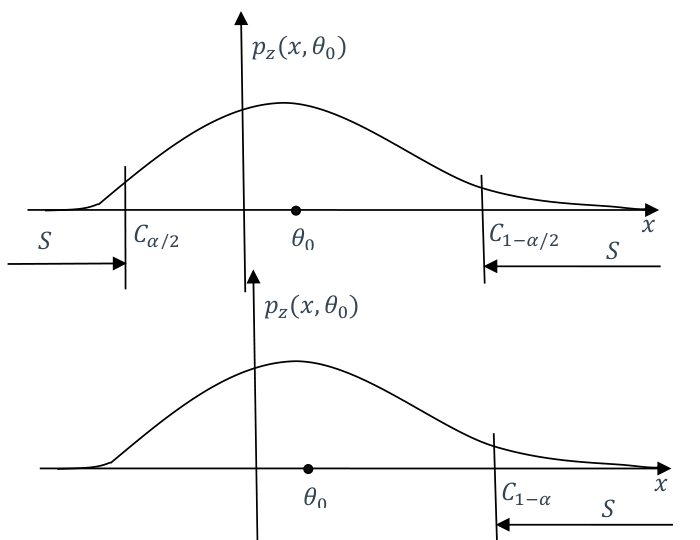
\includegraphics[width=0.8\textwidth]{Figures/9-plot1.png}
	\caption{}
	%FIXME: исправить описание
	\label{fig:9-plot1-png}
\end{figure}

\subsubsection{Ошибка первого рода}
\begin{definition}
	Условную вероятность 
	\[
			\alpha := P(z\in S \mid H_0)
	\]
назовём \emph{ошибкой первого рода}. Эта вероятность суть вероятность отклонения
верной гипотезы, \emph{уровень значимости критерия}.
\end{definition}
% отсебятина
Понятно, что чем уровень значимости критерия меньше, тем лучше сам критерий.
Понятно кроме того, что в реальных задачах критерий с нулевым уровнем
значимости существовать не может, поскольку он характеризует уже не гипотезу, а
некоторое верное утверждение и тем
самым теряет свой смысл.
 
Пусть $ H_0 $: $ \theta = \theta_0 $ --- простая гипотеза. Вид критического
множества для $ H_1 $: $ \theta \neq \theta_0 $ --- двусторонняя альтернатива.

Тогда  
\[
	S = \{z \leqslant C_{\alpha/2}\} \cup \{z \geqslant C_{1-\alpha/2}\}.
\]
В случае, когда альтернатива будет $ H_1 $: $ \theta > \theta_0 $
правосторонней, имеем  
\[
	S = \{z \geqslant C_{1-\alpha}\}.
	%FIXME: пропущено деление на два (\alpha/2)?
\]

\begin{ex}
	Пусть сопротивление резисторов $ \xi $ --- случайная величина, подчиняющаяся
	нормальному закону. Произведено $ n = 36 $
измерений, в результате чего оказалось, что $\bar X$ = 9.3\,кОм. 

Требуется проверить на уровне значимости $ \alpha = 0.05 $ гипотезу $ H_0 $: $ a = 10
$\,кОм против двусторонней альтернативы $ H_1 $: $ \theta \neq 10 $\,кОм в двух
ситуациях: а) $ \sigma^2 = 4 $\,кОм^2; b) $ S^2 = 6.25 $\,кОм^2.
\begin{solution}
	\begin{enumerate}[label=\alph*)] %TODO: буквы
	\item Как известно, статистика 
	\[
		\frac{\bar X - a}{\sigma}\cdot\sqrt{n}
	\]
	имеет стандартное нормальное распределение, то есть  
	\[
		P\left(u_{\alpha/2} \leqslant \frac{\bar X - a}{\sigma} \cdot \sqrt n \leqslant
		u_{1-\alpha/2} \right) = 1 - \alpha,
	\]
	или с учётом симметричности $ u_{\alpha/2} = -u_{1 - \alpha/2} $ нормального
	распределения  
	\[
			P \left( \left| \frac{\bar X - a}{\sigma}\cdot \sqrt n \right| \geqslant
			u_{1-\alpha/2} \right) = \alpha.
	\]

	Таким образом, поскольку $ u_{0.975} = 1.96 $, критическое множество в данном случае имеет вид
\[
		S = \left\{  \left| \frac{\bar X - a}{\sigma} \cdot \sqrt n \right| \geqslant
		u_{1-\alpha/2}\right\} = \left\{ \left| \frac{\bar X - 10}{2} \cdot 6 \right|
	\geqslant u_{0.975} \right\} = \{ \bar X \geqslant 10.65\} \cup \{\bar X
\leqslant 9.35\}.
\]
Поскольку $ \bar X = 9.3 \in S $, то гипотеза $ H_0 $: $ a = 10 $\,кОм
отклоняется на уровне значимости 0.05.
\item В этом случае используем статистику	 
\[
		\frac{\bar X - a}{S}\sqrt n,
\]
распределённую по закону Стьюдента, который также симметричен. Тогда 
\begin{align*}
	1 - \alpha &= P \left( t_{\alpha/2}(n-1)\leqslant \frac{\bar X - a}{S}\sqrt n
	\leqslant t_{1-\alpha/2}(n-1) \right),\\
	\alpha &= P \left( \left| \frac{\bar X - a}{S}\sqrt n \right| \geqslant
	t_{1-\alpha/2} (n-1) \right).
\end{align*}

Высчитав значение квантилли $ t_{0.975}(35) = 2.03 $, получим 
\[
		S = \left\{ \left| \frac{\bar X - a}{S}\sqrt n \right| \geqslant
		t_{1-\alpha/2}(n-1) \right\} = \left\{ \left| \frac{\bar X - 10}{2.5}\cdot 6
	\right| \geqslant 2.03 \right\} = \{\bar X \geqslant 10.84\} \cup \{\bar X
	\leqslant 9.15\}.
\]
В этом случае гипотеза $ H_0 $: $ a = 10 $\,кОм принимается, поскольку $ \bar X
= 9.3 \notin S$.
\end{enumerate}

\end{solution}
\end{ex}
\begin{ex}\label{ex:2}
	В условиях предыдущего примера требуется проверить на том же уровне значимости
	гипотезу $ H_0 $: $ a = 10 $\,кОм против левосторонней альтернативы $ H_1 $:
	$ a < 10 $\,кОм в двух ситуациях: a) $ \sigma^2 = 4 $\,кОм^2; b) $ S^2 = 6.25
	$\,кОм^2.
	\begin{solution}
		\begin{enumerate}[label=\alph*)]
			\item\label{enum:1} Решение этого примера  построено на той же статистике 
			\[
					\frac{\bar X - a}{\sigma}\sqrt n,
			\]
			однако критическое множество будет состоять из значений этой статистики,
			говорящих в пользу альтернативы, то есть 
			\[
				S = \left\{ \frac{\bar X - a}{\sigma}\sqrt n \leqslant - u_{1-\alpha}
				\right\} = \left\{ \frac{\bar X - a}{2} \cdot 6 \leqslant - 1.645
				\right\} = \{\bar X \leqslant 9.45 \}.
			\]
		Поскольку $ \bar X = 9.3 \in S $, то гипотеза $ H_0 $: $ a = 10 $\,кОм
		отвергается.	
	\item Аналогично предыдущему случаю, основную гипотезу нужно отвергать в случае малых 
		значений $X$. Произведем вычисления. Учитывая, что $ t_{0.95}(35) = 1.69 $,
	\[
		S = \left\{ \frac{\bar X - a}{S}\sqrt n \leqslant -t_{1-\alpha/2}(n-1)
		\right\} = \left\{ \frac{\bar X - 10}{2.5}\cdot 6 \leqslant -1.69 \right\} =
		\{\bar X \leqslant 9.296\}.
	\]
	В этом случае гипотеза $ H_0: a = 10 $\,кОм принимается, поскольку $ \bar X =
	9.3 \notin S$.
		\end{enumerate}

	\end{solution}
\end{ex}

\subsubsection{Ошибка второго рода}
\begin{definition}
Назовём условную вероятность
\[
	P(z\notin S \mid H_1) = \beta
\]
\emph{ошибкой второго рода}. Эта вероятность суть вероятность принятия неверной
гипотезы $ H_0 $ в случае простой альтернативы.
\end{definition}

\begin{definition}
Вероятность $W(S, \theta) = P_\theta(z\in S)$ называется \emph{функцией мощности
критерия}.
\end{definition}

При этом $ \alpha = W(S, \theta_0) $ --- вероятность отклонения верной гипотезы,
а $ 1-\beta = P(z \in S \mid H_1) = W(S, \theta_1) $ --- вероятность отвергнуть
неверную гипотезу.
%TODO: пояснить

%TODO: examples
\begin{ex}
	Требуется в условиях предыдущего примера проверить на том же уровне значимости
	ту же гипотезу $ H_0 $: $ a = 10 $\,кОм $ = a_0 $ против простой альтернативы
	$ H_1 $: $ a = 9 $\,кОм $ = a_1 $, если $ \sigma^2 = 4 $\,кОм^2. 
	\begin{solution}
		Поскольку $ a_1 < a_0 $, критическое множество совпадает с найденным в
		примере \ref{ex:2} п. \ref{enum:1}:  
		\begin{equation}\label{eq:1}
			S = \{\bar X \leqslant 9.45\},
		\end{equation}
		что даёт основания отвергнуть $ H_0 $ и принять $ H_1 $. 

		Вычислим ошибку	второго рода: 
		\begin{multline*}
				\beta = P(z \notin S \mid H_1) = P(\bar X > 9.45 \mid a = 9) =\\= P \left(
				\frac{\bar X - a}{\sigma}\sqrt n > \frac{9.45 - a}{\sigma}\sqrt n \mid a
			= 9\right) = P \left( \frac{\bar X - 9}{2} \cdot 6 > 1.35 \right) = 1 -
			\Phi(1.35) = 0.0885.
		\end{multline*}

	\end{solution}
\end{ex}
\begin{ex}
	В условиях предыдущего примера для того же уровня значимости требуется найти
	ошибку второго рода при проверке гипотезы $ H_0 $: $ a =10 $\,кОм $ = a_0 $
	против простой альтернативы $ H_1 $: $ a = 9.5 $\,кОм $ = a_1 $, если $
	\sigma^2 4 $\,кОм^2.
	\begin{solution}
		Поскольку $ a_1 < a_0 $, критическое множество будет тем же \eqref{eq:1},
		что даёт основания отвергнуть $ H_0 $ и принять $ H_1 $.

		Вычислим ошибку второго рода: 
		\[
				\beta = P(z\notin S\mid H_1) = P(\bar X > 9.45 \mid a = 9.5) = P \left(
				\frac{\bar X - a}{\sigma}\sqrt n> \frac{9.45 - a}{\sigma} \sqrt n\mid a
			= 9.5\right) = P \left( \frac{\bar X - 9}{2}\cdot 6 > -0.15 \right) =
			\Phi(0.15) = 0.56.
		\]

	\end{solution}	
\end{ex}
\begin{ex}
	В условиях предыдущих примеров для того же уровня значимости требуется найти
	функцию мощности левостороннего критерия при проверке гипотезы $ H_0 $: $ a =
	10$\,кОм $ = a_0 $ против простой альтернативы $ H_1 $: $ a = a_1 < a $, если
	$ \sigma^2 = 4 $\,кОм^2.
\begin{solution}
	По определению мощность критерия \eqref{eq:1} против альтернативы $ H_1 $: $ a
	= a_1 < 10$ можно вычислить следующим образом: 
	\[
			W(S, a_1) = P(\bar X \leqslant 9.45\mid H_1) = P \left( \frac{\bar X -
			a_1}{\sigma} \sqrt n \leqslant \frac{9.45 - a_1}{\sigma} \sqrt n \right) =
			\Phi = \left( \frac{9.45 - a_1}{\sigma}\sqrt n \right).
	\]
	\begin{figure}[h!]
		\centering
		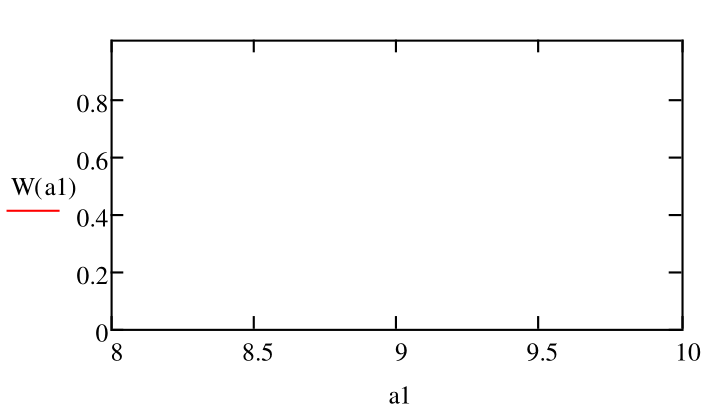
\includegraphics[width=0.8\textwidth]{Figures/9-plot2.png}
		\caption{}
		\label{fig:9-plot2}
	\end{figure}
	%FIXME: странный рисунок

\end{solution}
\end{ex}

\textsc{Вывод}.
Для построенного критерия в случае простой альтернативы ошибка второго рода 
вычисляется однозначно. 
 Большая ошибка второго рода говорит о низкой мощности критерия, он плохо различает 
близкие гипотезы. 

\subsubsection{Возможные задачи}
\begin{enumerate}
	\item Для данной альтернативы найти максимально мощный (оптимальный) критерий
		$ S^\ast $, то есть  
		\[
				W(S^\ast, \theta) = \max_S W(S,\theta).
		\]
	\item Для построенного критерия выбрать такую альтернативу, чтобы достигнуть
		максимальной мощности.
	\item Найти необходимый объём выборки, обеспечивающий заданную мощность
		критерия при заданных основной и альтернативной гипотезах.
\end{enumerate}


\subsection{Улучшение критерия за счёт увеличения объёма наблюдений}
Положим требуется найти минимальный объём выборки, удовлетворяющей условиям 
\begin{align*}
	H_0: a &= 10\text{\,кОм} = a_0,\\
	H_1: a &= 9.5\text{\,кОм} = a_1 < a_0,\\
	\sigma^2 &= 4\text{кОм}^2,\\
	\alpha &= 0.05, \quad \beta\leqslant0.1.
\end{align*}
\begin{solution}
	В рассматриваемой ситуации критическое множество имеет вид $ S = \{\bar X
	\leqslant C\} $. По условию 
	\begin{align*}
		0.05 &= P(z\in S\mid H_0) = P(\bar X \leqslant C \mid a = 10) = \Phi \left(
			\frac{C - 10}{2} \sqrt n\right),
			0.1 &\geqslant P(z \in \bar S \mid H_1) = P(\bar X > C \mid a = 9.5) = 1 -
		\Phi \left( \frac{C - 9.5}{2}\sqrt n \right).
	\end{align*}
Решая эту систему, находим $ n \geqslant 138 $.
\end{solution}

\textsc{Вывод}.  При увеличении числа наблюдений хорошая оценка (например та, для которой 
выполнены достаточные условия состоятельности $\D \widehat \theta_n \to 0$) по
вероятности (а значит, и 
по распределению) сходится к истинному значению параметра, то есть к неслучайной 
величине, что позволяет различить даже близкие простые гипотезы. 


\subsection{Оптимальный критерий Неймана -- Пирсона}
	С каждым критерием $ S $ свяжем функцию  
	\[
		\varphi(\vec X_n) = \begin{cases} 1, &z(\vec X_n) \in S,\\
		0, &z(\vec X_n) \notin S.\end{cases}
	\]
Тогда  
\begin{gather*}
	W(S, \theta) = W(\varphi(\vec X_n), \theta) = P_\theta(z(\vec X_n) \in S) =
	M_\theta(\varphi(\vec X_n)) = \int \varphi(\mathbf x) p(\mathbf x,
	\theta)\,d\mathbf x,\\
	W(S,\theta_0) = \alpha, \qquad W(S,\theta_1) = 1 - \beta.
\end{gather*}

\begin{theorem}[критерий отношения правдоподобия]\label{th:N-P}
	Рассмотрим множество критериев уровня $ \alpha $ для проверки гипотезы $ H_0
	$: $ \theta = \theta_0 $ против простой альтернативы $ H_1 $: $ \theta =
	\theta_1 $, $ \theta_1 \neq \theta_0 $. Тогда для любого $ 0 < \alpha < 1 $
	существуют такие числа $ c \geqslant 0 $ и $ \varepsilon \in [0, 1] $, что
	критерий с функцией  
	\[
	\varphi^\ast(\vec X_n) = \begin{cases} 1, & \frac{\mathscr L(\vec X_n,
		\theta_1)}{\mathscr L(\vec X_n, \theta_0)} > c,\\[0.4em]
		\varepsilon, & \frac{\mathscr L(\vec X_n, \theta_1)}{\mathscr L(\vec X_n, \theta_0)} =
		c,\\[0.4em]
		0, & \frac{\mathscr L(\vec X_n, \theta_1)}{\mathscr L(\vec X_n, \theta_0)} < c
	\end{cases}
	\]
является оптимальным (наиболее мощным) во множестве критериев уровня $ \alpha $.	
\end{theorem}
\begin{proof}
%TODO: proof
\end{proof}

\begin{ex} 
	Пусть выборка объёма $ n = 100 $ подчинена показательному закону с параметром
	$ \lambda $. Установим вид оптимального критического множества для проверки
	гипотезы $ H_0 $: $ \lambda = \lambda_0 $ против простой альтернативы $ H_1 $:
	$ \lambda = \lambda_1 $, если $ \lambda_1 > \lambda_0 $.
  \begin{solution}
		Согласно теореме \ref{th:N-P} оптимальное критическое множество имеет вид 
		\[
				\frac{\mathscr L(\vec X_n, \lambda_1)}{\mathscr L(\vec X_n, \lambda_0)} > c,
		\]
		откуда  
		\[
				\frac{\mathscr L(\vec X_n, \lambda_1)}{\mathscr L(\vec X_n, \lambda_0)} =
				\frac{\prod^n_{k=1} \lambda_1 e^{-\lambda_1 X_k}}{\prod_{k=1}^n
				\lambda_0 e^{-\lambda_0 X_k}} = \left( \frac{\lambda_1}{\lambda_0}
			\right)^n \exp\left[-\left(\lambda_1 - \lambda_0\right) \sum_{k=1}^n X_k\right] \geqslant c.
		\]
		Разрешим это неравенство относительно $ \sum_{k=1}^n X_k $ (достаточная
		статистика!): 
		\begin{align*}
				\exp\left[-\left(\lambda_1 - \lambda_0\right) \sum_{k=1}^n X_k\right]
				&\geqslant c \left( \frac{\lambda_0}{\lambda_1} \right)^n,\\
        -(\lambda_1 - \lambda_0) \sum_{k=1}^n X_k &\geqslant \ln \left[ c \left(
				\frac{\lambda_0}{\lambda_1}\right)^n  \right],\\
						\sum_{k=1}^n X_k &\leqslant \frac{\ln c + n \ln
				(\lambda_0/\lambda_1)}{\lambda_0 - \lambda_1} = c_1.
		\end{align*}

	\end{solution}	
\end{ex}

\begin{ex}
	\begin{enumerate}
		\item Построим критерий на уровне $ 1 - \alpha = 0.95 $ для различения
			гипотез о параметре показательного закона на основе выборки объёма $ n =
			100 $, где 
			\begin{align*}
				H_0: \lambda &= \frac{1}{3},\\
				H_1: \lambda &= \frac{5}{11}.
			\end{align*}
			\begin{solution}
				Согласно критерию Неймана -- Пирсона $ S = (\bar X \leqslant C) $.
				Далее, 
				\[
						\alpha = P(\bar X \in S \mid H_0 ) = P(\bar X \leqslant C \mid H_0)
						= P \left( 2\lambda_0 \sum_{k=1}^n X_k \leqslant 2\lambda_0 n C
						\right) = F_{\chi^2(2n)}(2\lambda_0 n C).
				\]
				Значит, $ 2\lambda_0 n C = \chi^2_\alpha(2n) $, а значит, 
				\[
						C = \frac{\chi^2_\alpha(2n)}{2\lambda_0 n} = 2.524.
				\]

			\end{solution}
			
			\item Найдём ошибку второго рода построенного критерия.
				\begin{solution}
				\[
					\beta = P(\bar X > C \mid H_1 ) = P \left( 2\lambda_1 \sum_{k=1}^n X_k
					> 2\lambda_1 n C\right) = 1 - F_{\chi^2(2n)}(2\lambda_0 n C) = 0.075.
				\]

			\end{solution}

		\item Найдём объём выборки, обеспечивающий при решении задачи о различении
			этих гипотез ошибки $ \alpha = 0.05 $ и $ \beta = 0.05 $.

			\begin{solution}
			Согласно критерию Неймана -- Пирсона $ S = (\bar X \leqslant C) $. Тогда
			при больших $ n $ имеем  
			\begin{align*}
				\alpha &= P(\bar X \in S\mid H_0) = P(\bar X \leqslant C \mid H_0) = P
					\left( \frac{n\bar X - 1/\lambda_0}{\sqrt{n/\lambda^2_0}}\leqslant
					\frac{nC - n/\lambda_0}{\sqrt{n/\lambda^2_0}} \right) \approx \Phi
					\left( \frac{n C \lambda_0 - n}{\sqrt n} \right),\\ 
				\beta &= P(\bar X \notin S \mid H_1) = P(\bar X > C \mid H_1) = P
					\left( \frac{n\bar X - 1/\lambda_1}{\sqrt{n/\lambda^2_1}}\leqslant
					\frac{nC - n/\lambda_1}{\sqrt{n/\lambda^2_1}} \right) \approx \Phi
					\left( \frac{n C \lambda_1 - n}{\sqrt n} \right).
			\end{align*}
			
			Решим полученную систему: 
			\[
				\begin{cases}
					C \lambda_0 \sqrt n - \sqrt n = u_\alpha,\\
					C\lambda_1 \sqrt n - \sqrt n = u_{1-\beta}.
				\end{cases}
				\implies
				\begin{cases}
					\sqrt n = \frac{u{1-\beta}\lambda_0 - u_\alpha \lambda_1}{\lambda_1 -
					\lambda_0},\\
					C = \frac{\sqrt n + u_\alpha}{\lambda_0\sqrt n}.
				\end{cases}
				\implies
				\begin{cases}
					n \approx 115, \\
					C = 2.538.
				\end{cases}
			\]

		\end{solution}
	\end{enumerate}
\end{ex}
	

	\section{Лекция 10 - 2023-11-08 - }

% TODO начало я пропустил - дописать

% TODO кажется это доказательство всё-таки относиться к прошлой лекции

\subsection{Критерии отношения правдоподобия}

\begin{theorem}[Неймана-Пирсона]
  $\vec{X}_n = (X_1, X_2,\dots, X_n) \sim F(x, \theta)$ тогда критерий уровня $\alpha$ $(S^*, Z(\vec{X}_n)) = \dfrac{\mathcal{L} (\vec{X}_n, \theta_1)}{\mathcal{L}(\vec{X}_n, \theta_0)}$, тогда $\forall 0 < \alpha < 1 \exists \varepsilon \in [0, 1] : \varphi^*(\vec{X}_n) = \begin{cases}
    1, &z > C \\
    \varepsilon, &z=C \\
    0, &z<C
  \end{cases}
  $ - является оптимальным среди всех критериев с заданной $\alpha$
  
  т.е. $\forall$ крит функции $\tilde S$ с $\tilde \varphi$ уровня $\alpha$ $W(S^*, \theta_1) \geqslant W(\tilde S, \theta_1)$ $\Rightarrow$ ошибка $\beta$ меньше.
\end{theorem}

% TODO причем само доказатльетсво я не успел


\begin{ex}
  $X_1,\dots,X_n \sim N(a, \sigma)$, $a = a_0$ - известно
  $H_0 : \sigma = \sigma_0$
  $H_1 : \sigma = \sigma_1$
  \begin{multline*}
    \dfrac{L(\bar X, \sigma_1)}{L(\bar X, \sigma_0}
    = \prod \dfrac{\dfrac{1}{\sqrt{2\pi} \sigma_1} exp(- \dfrac{(x_k - a_0)^2}{2sigma_1^2})}{\dfrac{1}{\sqrt{2\pi} \sigma_0} exp(- \dfrac{(x_k - a_0)^2}{2sigma_0^2})}
    = (\dfrac{\sigma_0}{\sigma_1})^n exp(-\dfrac{1}{2\sigma_1^2} \sum (X_k-a_0)^2 + \dfrac{1}{2\sigma_0^2} \sum (X_k-a_0)^2 ) = \\
    = (\dfrac{\sigma_0}{\sigma_1})^n exp( -\dfrac{1}{2} \sum \dfrac{\sigma_0^2 (X_k-a_0)^2 + \sigma_1^2 (X_k - a_0)^2}{\sigma_1^2 \sigma_0^2} ) \geqslant C
  \end{multline*}

  \begin{equation*}
    (\dfrac{\sigma_0}{\sigma_1})^n exp(-1/2 \dfrac{\sigma_0^2 - \sigma_1^2}{\sigma_1^2 \sigma_0^2} \sum (X_k-a_0)^2) \geqslant C
  \end{equation*}

  На основе знания какая из сигм больше можно уже построить критерий вида:
  $$ S = \{ \sum(X_k-a_0)^2 \leqslant (\geqslant) C_1 \} $$
\end{ex}

\subsection{Графическая иллюстрация критерия отношения правдоподобия}

% TODO здесь картинка

\subsection{Графическая иллюстрация критерия Вальда}

% TODO рисунок из её лекций на странице 10

Снизу область принятия $H_0$, сверху область принятия $H_1$ посередине область продолжения наблюдений. Как только после очередного наблюдения статистика перешла вниз или вверх, наблюдения прекращаются и принимается нужная гипотеза.

Статистика критерия $(\nu, X_1, X_2, \dots, X_n)$
$\nu = min \{ n : Z_n \notin (B, A) \}$, $z_n = \dfrac{L(X_1, \dots, X_n, \theta_1)}{L(\bar X, \theta_0)}$

Критерий: Пусть 0<B<1<A.
$z_\nu \geqslant A$ - принимаем $H_1$; $z_\nu \leqslant B$ - принимаем $H_0$.

\begin{theorem}
  $i = 0, 1; P_{\theta_i}(\nu < \infty) = 1, \exists M_{\theta_0} \nu < \infty, M_{\theta_1} \nu < \infty$

  Здесь $i = 0, 1; P_{\theta_i}$ означает, что при любой верной гипотезе эта вероятность $=1$
\end{theorem}

\begin{proof}
  Назовем $Y_k = \ln \dfrac{P(X_k, \theta_1)}{P(X_k, \theta_0)}$.

  $\ln Z_n = \sum \ln \dfrac{P(X_k, \theta_1)}{P(X_k, \theta_0)} = \sum Y_k$

  Зададим целое r, и:
  \begin{align*}
    \eta_1 &= Y_1 + Y_2 + \dots + Y_r \\
    \eta_2 &= Y_{r+1} + Y_{r+2} + \dots + Y_{2r} \\
           &\dots \\
    \eta_k &= Y_{(k-1) r + 1} + \dots + Y_{kr}
  \end{align*}

  Тогда событие $(\nu > rk)$ означает, что $(\ln B < Y_1 + \dots + Y_j < \ln A, j \leqslant rk)$, а следовательно и $(\ln B < \eta_1 + \eta_2 + \dots + \eta_j < \ln A, j \leqslant k)$.

  \begin{multline*}
    P(\nu > kr) = P(\ln B < Y_1 + \dots + Y_j < \ln A, j \leqslant kr) \leqslant \\
    \leqslant P(\ln B < \eta_1 + \eta_2 + \dots + \eta_i < \ln A, i \leqslant k) \leqslant \\
    \leqslant P(|\eta_i| < \ln A - \ln B, i \leqslant k)
    = P(\bigcap (|\eta_i| < \ln A - \ln B)) = \\
    \text{т.к. $\eta_i$ - назависимы и одинаково распределены} \\
    = (P_{\theta_i} (|\eta_i| < \ln (A/B)))^k
  \end{multline*}


  Выбираем r так, чтобы
  
  $\forall i : M \eta_i^2 \geqslant D \eta_i = r \cdot D Y_i > C^2 = (\ln (A/B))^2$
  
  $\Rightarrow P(\theta_i) = P_{\theta_i} (|\eta_i| < C) < 1$

  иначе $P_{\theta_i} (|\eta_i| < C) = 1 \Rightarrow M \eta_i^2 < C^2$

  $P_{\theta_i} (\nu > rk) \leqslant (P(\theta_i))^k = (P(\theta_i)^{1/r})^{rk}$

  $P_{\theta_i} (\nu > rk) \to 0, k \to \infty$

  $M_{\theta_i} \nu = \sum n P_{\theta_i} (\nu  = n) = \sum P_{\theta_i} (\nu \geqslant n) = \sum ( P(\theta_i)^{1/r} )^{nr}$

  Теорема доказана
\end{proof}

Вторая особенность такого критерия состоит в том, что он чувствителен к порядку учета выборки.

\begin{theorem}[Вальда]
  Если заданы A и B, то ошибки $\alpha$ и $\beta$ удовлетворяют неравенствам:
  \begin{equation*}
    \begin{cases}
      \dfrac{1 - \beta}{\alpha} \geqslant A \\[1em]
      \dfrac{\beta}{1 - \alpha} \leqslant B
    \end{cases}
  \end{equation*}
  (максимально широкий коридор)

  Эти неравенства называют тождестами Вальда.

  % TODO здесь еще рисуночек (в лекциях на странице 12)
\end{theorem}

Применение: если $\alpha$ и $\beta$ заданы, то берут $A = \dfrac{1-\beta}{\alpha}, B = \dfrac{\beta}{1 - \alpha}$
% TODO расписать в применении, почему берем именно крайние точки из неравенств
Почему так? - иначе сумма ошибок будет больше

\begin{proof}
  % TODO вместо X_0n лучше использовать каппу, а то путаница с переменными
  $X_{0n} = \left( \vec{X}_n : B < Z_k < A, k = \overline{1, n-1}, z_n \leqslant B \right)$ - множество тех, которые ведут к принятию гипотезы $H_0$
  $X_{1n} = \left( \vec{X}_n : B < Z_k < A, k = \overline{1, n-1}, z_n \geqslant A \right)$ - множество тех, которые ведут к принятию гипотезы $H_1$

  \begin{equation*}
    1 = \sum  P_{\theta_i} (\nu = n) = \sum P_{\theta_i} (X_{0n}) + \sum P_{\theta_i} (X_{1n}) = \\
    = \begin{cases}
      (1 - \alpha) + \alpha, &\theta_0 \\
      \beta + (1 - \beta), &\theta_1
    \end{cases} 
  \end{equation*}

  \[
    \alpha = \sum P_{\theta_0} (X_{1n}) \leqslant \dfrac{1}{A} \sum P_{\theta_1} (X_{1n}) = \dfrac{1 - \beta}{A}
  \]
  
  Рассмотрим почему среднее неравенство верно. Для дискретного случая:
  \[
    P_{\theta_1} (X_{0n}) = \sum_{\vec{X_n} \in X_{1n}} P_{\theta_1}(\xi_1 = X_1, \dots, \xi_n = X_n)= \sum \mathcal{L} (X_1, \dots, X_n, \theta_1) \leqslant \dfrac{1}{A} \sum \mathcal{L} (\dots, \theta_1) = \dfrac{1 - \beta}{A}
  \]

  \[
    \beta = \sum P_{\theta_1} (X_{0n}) = \sum_{n=1}^\infty \sum_{\vec{X}_n \in X_{0n}} P_{\theta_1} (\vec{\xi} = \vec{X}_n)
  \]
\end{proof}

	\section{Лекция 11 - 2023-11-15 - Непараметрические гипотезы. Критерий согласия $\chi^2$ Пирсона. Проверка гипотезы о виде распределения.}

Рассмотрим гипотезу: $H_0: X_1, \dots, X_n \sim F(x)$,
где $F(x)$ -- что-то очень конкретное, например $N(0, 1)$, $R[0, 2]$.
И тотальную альтернатива к ней $H_1$ - выборка не подчиняется $F(x)$.

Группированная выборка 
\begin{center}
  \begin{tabular}{|c|c|c|c|c|}
    \hline
    группированная выборка & E_1 & E_2 & \dots & E_n \\
    \hline 
    Эмп. частоты & \nu_1 & \nu_2 & \dots & \nu_n \\
    \hline 
    При $H_0$ - теор. частоты & np_1 & np_2 & \dots & np_m \\
    \hline
  \end{tabular}
\end{center}

Соотвественно, надо проверять похожи ли две эти строчки друг на друга.

Для оценки схожести вводятся различные метрики.
Пирсон придумал очень удачную метрику:
\[
  \chi^2_B = \sum_{k=1}^m \dfrac{(\nu_k - np_k)^2}{np_k}
\]

\begin{theorem}{Пирсона (для простых гипотез)}
  !! простая гипотеза означает, что закон распределения очень конкретный (без параметра)

  Пусть $E$ - множество значений $X_i$ представлено в виде: $E = \cup_{i=1}^m E_i$ % TODO в оригинале там квадратный \cup
  (объединение непересекающихся множеств $E_i \cap E_j = \emptyset$) 

  Пусть $p_i = P_0 (X_i \in E_i)$, $\nu_i$ - частоты попадения в $E_i$. Тогда:
  \[
    \chi^2_B = \sum \dfrac{(\nu_i - np_i)^2}{np_i} \toD \chi^2 (m-1), n \to \infty
  \]
  
\end{theorem}

\begin{proof}
  Напомним, что характеристическая функция это:
  \[
    f_\xi (t) = M e^{i t \xi}, f_{\bar \xi} = M e^{i \bar t^T \bar \xi} = M e^{i \sum t_k \xi_k}
  \]

  При 0-ой гипотезе:
  \[
    p_i = P_0 (\xi \in E_i)
  \]

  Ясно, что это распределено по полиномиальному закону:
  \[
    P(\bar \nu = (n_1, n_2, \dots, n_m)) = \dfrac{n!}{n_1! n_2! \dots n_m!} p_1^{n_1} p_2^{n_2} \dots p_m^{n_m}, \sum n_i = n
  \]

  \[
    \sum \dfrac{n!}{n_1! n_2! \dots n_m!} p_1^{n_1} \dots p_m^{n_m} = 1
  \]

  \begin{multline*}
    f_{\bar \nu} (\bar t) = M e^{i \bar t^T \bar \nu} =
    \sum e^{i \sum t_k n_k} \dfrac{n!}{n_1! n_2! \dots n_m!} p_1^{n_1} \dots p_m^{n_m} = \\
    = \sum \dfrac{n!}{n_1! n_2! \dots n_m!} (p_1 e^{i t_1})^{n_1} (p_2 e^{i t_2})^{n_2} \dots (p_m e^{i t_m})^{n_m} = 
    (p_1 e^{i t_1} + p_2 e^{i t_2} + \dots + p_m e^{i t_m})^n = \\
    = (1 + p_1 (e^{i t_1} - 1) + p_2 (e^{i t_2} - 1) + \dots + p_m (e^{i t_m} - 1))^n
  \end{multline*}

  \[
    \ln f_{\bar \nu} (\bar t) = n \ln (1 + p_1 (e^{i t_1} - 1) + p_2 (e^{i t_2} - 1) + \dots + p_m (e^{i t_m} - 1))
  \]

  Обозначим: 
  \[
    \eta_k = \dfrac{\nu_k - np_k}{\sqrt{np_k}}, \chi^2_B = \sum_{k=1}^m \eta_k
  \]

  Тогда
  \[
    f_{\bar \eta} (\bar t) = M e^{i \bar t^T \bar \eta} =
    M e^{i \sum t_k \dfrac{\nu_k - np_k}{\sqrt{np_k}}} = 
    M e^{i \sum \dfrac{t_k}{\sqrt{np_k}} \nu_k} \cdot e^{i \sum t_k \sqrt{np_k}} = 
    f_{\bar \nu} (\dfrac{t_1}{\sqrt{np_1}}, \dots, \dfrac{t_m}{\sqrt{np_m}}) e^{i \sum t_k \sqrt{np_k}}
  \]

  Тогда
  \[
    \ln f_{\bar \nu} (\bar t) = -i \sum t_k \sqrt{np_k} + n \ln (1+p_1 (e^{\dfrac{i t_1}{\sqrt{np_1}}} - 1)+ \dots + p_m (e^{\dfrac{i t_m}{\sqrt{np_m}}} - 1) )
  \]

  Используя эквивалентности:
  \begin{multline*}
    = -i \sum t_k \sqrt{np_k} + n \left( \sum p_k (e^{\dfrac{i t_k}{\sqrt{np_k}}} - 1) - \dfrac{1}{2} (\sum p_k(e^{\dfrac{i t_k}{\sqrt{np_k}}} - 1))^2 + o(\dfrac{1}{n}) \right) = \\
    = -i \sum t_k \sqrt{np_k} + n \left( \sum p_k (\dfrac{i t_k}{\sqrt{np_k}} + \dfrac{1}{2} \sum \dfrac{i t_k}{\sqrt{np_k}})^2 - \dfrac{1}{2} (\sum p_k \dfrac{i t_k}{\sqrt{np_K}})^2 + o(\dfrac{1}{n}) \right) = \\
    = - \dfrac{1}{2} \sum t_k^2 + \dfrac{1}{2} \left( \sum t_k \sqrt{p_k} \right)^2 + o\left(\dfrac{1}{n}\right)
    = - \dfrac{1}{2} \bar t^T \bar t + \dfrac{1}{2} ((C \bar t)_1)^2 + o(1)
  \end{multline*}
  где $C$ - ортогональное преобразование $\bar \xi = C \eta$, с первой строчкой $(\sqrt{p_1}, \dots, \sqrt{p_m})$,
    а индексом 1 в $(C \bar t)_1$ обозначено взятие первого элемента вектора.

  Рассмотрим, что происходит с характеристической функцией при ортогональных преобразованиях:
  \[
    f_{\bar \xi} (\bar t) = M e^{i \bar t^T \bar t} = M e^{i \bar t^T C \eta} =
    M e^{i (C^T \bar t)^T \bar \eta} = f_{\bar \eta} (C^T \bar t)
  \]

  \[
    \ln f_{\bar \xi} (\bar t) = - \dfrac{1}{2} (C^T \bar t)^T C^T \bar t + \dfrac{1}{2} ((C C^T \bar t))^2 + o(1) = -\dfrac{1}{2} \bar t^T \bar t + \dfrac{1}{2} t_1^2 + o(1) = - \dfrac{1}{2} \sum_{k=2}^m t_k^2 + o(1)
  \]

  \[
    \chi^2_B = \sum \dfrac{(\nu_k - np_k)^2}{np_k} = \sum \eta_k^2 = \bar \xi^T C^T C \bar \xi = \sum \xi_k^2
  \]

  Рассмотрим как распределен вектор $\bar \xi$:
  
  Если бы $\bar \xi \sim N(0, \Sigma)$, то:
  \[
    (\xi_1, \dots, \xi_m) \sim N(0, \Sigma) \Leftrightarrow f_{\bar \xi} (\bar t) = e^{-\dfrac{1}{2} \sum \sigma_k^2 t_k^2}
  \]

  В нашей ситуации выходит, что $\sigma_1 = 0$, следовательно, $\sum \xi_k^2 \sim \chi^2 (m-1)$.
\end{proof}

Применение: если $np_k$ достаточно большие (на практике $np_k \geqslant 5$). Тогда не выполняется предельные условия в теореме (как минимум условия ЦПТ). Иначе следует объединять $E_k$ с соседними.

Соответственно, формулируем критерий:

Если $\chi^2_B \geqslant \chi^2_{1-\alpha} (m-1)$, то $H_0$ отклоняем.

Если $\chi^2_B < \chi^2_{1-\alpha}(m-1)$, то $H_0$ принимаем.

\begin{ex}[Мендель]
  556 горошин скрещивали во втором поколении.

  В первом поколении все оказались желтыми.

  Доминантный ген означает, что если от родителей достались два разных гена,
  то проявляться будет именно доминантный.
  
  \begin{center}
    \begin{tabular}{|c|c|c|c|c|}
      \hline
       & Круглые и желтые & кругл. зелен & морщинистые и желт & морщинис. и зел \\
      \hline
      частоты & 315 & 108 & 101 & 32 \\
      \hline
      $np_k$ & $\dfrac{9}{16} 556$ & $\dfrac{3}{16} 556$ & $\dfrac{3}{16} 556$ & $\dfrac{1}{16} 556$ \\
      \hline
    \end{tabular}
  \end{center}

  $H_0$ - гипотеза о том, что признаки цвета и формы независимы,
  а круглая форма и желтный цвет - доминантные признаки.

  Посчитаем $\chi^2_B$ и применим критерий:
  \[
    \chi^2_B = 0.47 < \chi^2_{0.9} (3) = 6.25
  \]
  получаем, что $H_0$ - верна.
\end{ex}

  \section{Лекция 12 - 2023-11-22 - Непараметрические гипотезы}

\subsection{Критерий Фишера для сложных гипотез}

\begin{ex}
  Случай сложной гипотезы
  $X_1, X_2, \dots, X_n \sim F(x, \bar \theta)$, $\bar\theta = (\theta_1, \dots, \theta_r)$.

  Гипотеза $H_0$ - выборка подчиняется закону $F$.
\end{ex}

\begin{theorem}[Теорема Фишера (критерий Фишера для сложных гипотез)]
  Пусть проверятеся гипотеза $H_0$ - выборка из закона $F(x, \bar\theta)$.
  
  Пусть множество значений СВ $E = E_1 + \dots + E_l$.
  
  Пусть $p_l (\bar\theta) = p(\xi \in E_l) = \int_{E_l} dF(x, \bar\theta)$. 
  $\hat{\bar\theta}$ - ОМП параметра $\bar\theta$.
  Тогда если
  \[
    \exists \dfrac{\partial p_l(\bar\theta)}{\partial \theta_i}, \dfrac{\partial^2 p_l(\bar\theta)}{\partial \theta_i \partial \theta_j}, i, j = \overline{1, r}; k=\overline{1, l},
  \]
  А матрица $\left(\dfrac{\partial p}{\partial \bar\theta}\right)$ - имеет ранг r, то
  \[
    \chi^2_B = \sum_{k=1}^l \dfrac{(\nu_k - np_k(\hat{\bar\theta}))}{np_k(\hat{\bar\theta})} \toD \chi^2 (l-1-r)
  \]
\end{theorem}

Замечание: условия теоремы не выполнены например для выборки $X_1, \dots, X_n \sim R[a, b]$.
ОМП: $\hat a = X_{(1)}, \hat b = X_{(n)}$. $p_k (a, b) = \int_{E_k} \dfrac{1}{b-a} dx$ - не является дифф. (в точках a и b скачки).

При использовании критерия считают $r = 0$.

Критерий: $\chi^2_B \geqslant \chi^2_{1-\alpha} (l-1-r)$, то $H_0$ отклоняют, если $\chi^2_B < \chi^2_{1-\alpha} (l-1-r)$, то $H_0$ принимается.

\begin{ex}
  537 снарядов упало на Лондон. Территорию Лондона разделили на 576 участков по 0.25 км.

  \begin{center}
    \begin{tabular}{|c|c|c|c|c|c|c|}
      \hline
      снаряды $k_j$ & 0 & 1 & 2 & 3 & 4 & 7 \\
      \hline
      участки $\nu_j$ & 229 & 211 & 93 & 35 & 7 & 1 \\
      \hline
      n \hat{p_j} & 226.74 & 211.39 & 98.54 & 30.62 & 8.71 \\ 
      \hline
    \end{tabular}
  \end{center}

  Гипотеза $H_0$ - число снарядов на 1 участок $\sim Pois$.

  \[
    p(\xi = k) = \dfrac{\lambda^k}{k!} e^{-\lambda}.
  \]

  ОМП $\hat \lambda = \bar X = \dfrac{537}{576}$. Считаем $\hat{p_0} = e^{-537 / 576}, \dots$.
  Столбцы 4 и 7 пришлось объединить, так как $n\hat{p_4} < 5$.

  \[
    \chi^2_B \approx 1.5; \chi^2_{0.95} (5-1-r) = \chi^2_{0.95} (3) = 7.81,
  \]

  Критерий имеет вид: $S = \{ \chi^2_B > \chi^2_{0.95}(3) \}$, $\chi^2_B \notin S \Rightarrow H_0$ -- принимается.
\end{ex}

\begin{ex}
  Проверка гипотезы о независимости признаков.

  $X_1, \dots, X_n$ обладают признаками A и B.
  Признак A имеет m градаций, а признак B имеет k градаций.

  Таблица сопряженности признаков

  \begin{center}
    \begin{tabular}{|c|c|c|c|c|}
      \hline
      A_i \ B_i & B_1 & B_2 & \dots & B_k \\
      \hline
      A_1 & \nu_{11} & & & \\
      \hline
      \dots & \dots & & & \\
      \hline
      A_m & & & & \\
      \hline
    \end{tabular}
  \end{center}

  $\nu_{ij}$ - кол-во элементов выборки, обладающие признаками $A_i, B_j$.

  Гипотеза: $H_0$ признаки A и B независимы.
  \[
    P(A_i B_j) = P(A_i) P(B_j)
  \]

  \[
    \dfrac{\nu_{ij}}{n} \approx \dfrac{\nu_i}{n} \dfrac{\nu_j}{n},
  \]
  где $\nu_i = \sum_j v_{ij}$, $\nu_j = \sum_i v_{ij}$.

  \[
    \chi^2_B = \sum_{i=1}^m \sum_{j=1}^k \dfrac{(\nu_{ij} - n \hat p_{ij})^2}{n \hat p_{ij}}
  \]

  Параметры: $P(A_1), P(A_2), \dots, P(A_m); \sum P(A_i) = 1$, следовательно, независимых параметров здесь $m-1$. $P(B_1), P(B_2), \dots, P(B_k); \dots$, следовательно, независимых параметров $k-1$. Вместе параметров $r = m+k-2$.

  \[
    \hat p_{i} = P(A_i) = \dfrac{\nu_i}{n}; \hat p_j = P(B_j) = \dfrac{\nu_j}{n}.
  \]

  При $H_0$:
  \[
    \hat p_{ij} = \hat p_i \cdot \hat p_h = \dfrac{\nu_i \nu_j}{n^2}
  \]

  \begin{multline*}
    \chi^2_B
    = \sum_{i=1}^m \sum_{j=1}^k \dfrac{(\nu_{ij} - n \hat p_{ij})^2}{n \hat p_{ij}}
    = n \sum_{i=1}^m \sum_{j=1}^k \dfrac{\nu^2_{ij}}{\nu_i \nu_j} - 2 \sum_{i=1}^m \sum_{j=1}^k \nu_ij + n \sum_{i=1}^m \sum_{j=1}^k = \\
    = n \sum_{i=1}^m \sum_{j=1}^k \dfrac{\nu^2_{ij}}{\nu_i \nu_j} - 2n + n
    = n \left(\sum_{i=1}^m \sum_{j=1}^k \dfrac{\nu^2_{ij}}{\nu_i \nu_j} - 1\right)
  \end{multline*}

  Число степеней свободы

  $l-1-r = k m - 1 - (m+k-2) = (k-1)(m-1)$

  Критерий: $\chi^2_B \geqslant \chi^2_{1-\alpha} ( (k-1)(m-1) )$, то $H_0$ принимается;
  если $\chi^2_B < \chi^2_{1-\alpha} ( (k-1)(m-1) )$.
\end{ex}

\begin{ex}
  100 студентов проходили опрос мешает ли курение учёбе.
  В зависимости от курса были получены данные:

  \begin{center}
    \begin{tabular}{|c|c|c|c|c|}
      \hline
      ответ / курс & 1 курс & 2 курс & 3 курс & $ \Sigma $ \\
      \hline
      нет & 15 & 10 & 0 & 25\\
      \hline
      не знаю & 8 & 5 & 7 & 20 \\
      \hline
      да & 0 & 30 & 25 & 55 \\
      \hline
      $ \Sigma $  & 23 & 45 & 32 & 100 \\
      \hline
    \end{tabular}
  \end{center}

  Проверить гипотезу $H_0$ о том, что мнение не зависит от курса.
  \[
  \chi^2_B = 100 (\dfrac{15^2}{25*23} + \dfrac{10^2}{45*25} + \dots + \dfrac{25^2}{55*32} - 1) = 44.2
  \]

  Не забываем про условие применимости: $\dfrac{\nu_i \nu_j}{n} \geqslant 4$.

  $\chi^2_{0.95} = 13.3$ следовательно $H_0$ отклоняем.
\end{ex}

\subsection{Критерий согласия Колмогорова}

\begin{theorem}
  $X_1, \dots, X_n \sim F(x)$.

  Выборочная функция распределения:
  \[
    \hat{F}_n(x) = \dfrac{1}{n} \sum_{k=1}^n I(x-X_k)
  \]

  Если $F(x)$ непрерывна, то закон распределения статистики Колмогорова $D_n = \sup_x |\hat{F}_n(x) - F(x)|$ - не зависит от вида $F(x)$.
\end{theorem}

\begin{proof}
  Пусть $F(x)$ - строго монотонна. Перейдем от выборки $X_k$ к выборке $Y_k$ по правилу:
  \[
    X_1, \dots X_n \to Y_1, \dots, Y_n; Y_k = F(X_k)
  \]

  $\dfrac{1}{n} \sum_{k=1}^n I(X_k < F^{-x} (y)) = \dfrac{1}{n} \sum_{k=1}^n I(Y_k < y)$

  \begin{multline*}
    D_n = \sup_{-\infty < x < \infty} |\hat{F}_n(x) - F(x)|
    = \left|\, \begin{aligned}
      x = F^{-1} (y) \\
      (-\infty, \infty) \to [0, 1]
    \end{aligned} \,\right|\\ 
    = \sup_{0 \leqslant y \leqslant 1} |\hat{F}_n (F^{-1} y) - F(F^{-1} (y))|
    = \sup_{0\leqslant y \leqslant 1} |\hat{F}_n(y) - y|
  \end{multline*}

  Условие строгой монотонности можно опустить, потому что достижение супремума всё равно достигается на участках строгой монотонности.
\end{proof}

О вычислении $D_n$:
\[
  X_1, \dots, X_n \to Y_1, \dots, Y_n; Y_k = F(X_k).
\]
Построим вариационный ряд
\[
  Y_{(1)} \leqslant \dots \leqslant Y_{(n)}
\]

\[
  D_n = \sup_{y \in [0, 1]} |\hhat{F}_n(y - y|
  = \max_{1\leqslant k \leqslant n} \max | |Y_{(k) - \dfrac{k}{n}}|, |Y_{(k)} - \dfrac{k-1}{n}| |
  = \max_{1 \leqslant k \leqslant n} \{ |Y_{(k)} - \dfrac{2k-1}{2n}| + \dfrac{1}{2n} \}
\]

Потому что максимум разности $\hhat{F}_n(y) - y$ достигается в точках скачков ЭФР.

Для критерия Колмогорова важно чему равен объем выборки: $n\leqslant 35$ (иначе используем предельные теоремы).

Основная гипотеза: $H_0:$ выборка подчинается закону $F(x)$.

Критерий: $D_n \geqslant K_{1-\alpha} (n)$ - $H_0$ отклоняем.
  $D_n < K_{1-\alpha} (n)$ - $H_0$ принимаем. 

$K_{1-\alpha} (n)$ - значения D-критерия Колмогорова-Смирнова.

\begin{ex}
  Пассажир замерял время ожидания автобуса в минутах: $X_k = \{ 5.1; 3.7; 1.2; 9.2; 4.8 \}$.
  Проверить гипотезу $H_0$ о том, что время ожидания $\sim R[0, 10]$.
 
  Упорядочим выборку:
  \[
    X_{(k)} = \{ 1.2, 3.7, 4.8, 5.1, 9.2 \}
  \]

  Для равномерного закона функция распределения:
  \[
    F(x) = \dfrac{x}{10}
  \]

  \begin{center}
    \begin{tabular}{|c|c|c|c|}
      \hline
      $X_{(k)}$ & $Y_{(k)}$ & $\dfrac{2k-1}{2n}$ & $\left| Y_{(k)} - \dfrac{2k-1}{2n} \right| + \dfrac{1}{2n}$ \\
      \hline
      1.2 & 0.12 & 0.1 & 0.12 \\
      3.7 & 0.37 & 0.3 & 0.17 \\
      4.8 & 0.48 & 0.3 & 0.12 \\
      5.1 & 0.51 & 0.7 & 0.29 \\
      9.2 & 0.92 & 0.9 & 0.12 \\
      \hline
    \end{tabular}
  \end{center}

  \[
    D_5 = 0.29
  \]

  Значение $K_{0.95} (5) = 0.56$, следовательно, $H_0$ принимаем.
\end{ex}

\subsection{Критерий Колмогорова для $k>35$}

\begin{theorem}[Критерий Колмогорова для $k>35$]
  Пусть $K(x) = \sum_{j=-\infty}^{\infty} (-1)^j e^{-2j^2 x^2}, x>0$.

  $\forall F(x) \in C$ статистика $\sqrt{n} D_n$ при $n\to\infty$ сходится по распределению к $K(x)$:
  \[
    \lim_{n\to\infty} (\sqrt{n} D_n < x) = K(x)
  \]

  % TODO рисунок сени тут должен быть он обещал

  Критерий: $\sqrt{n} D_n \geqslant \lambda_{1-\alpha}$, то $H_0$ отклоняется. Если $\sqrt{n} D_n < \lambda_{1-\alpha}$, то $H_0$ - принимается.

  \begin{center}
    \begin{tabular}{|c|c|c|c|c|}
      \hline
      $1-\alpha$ & 0.9 & 0.95 & 0.98 & 0.99 \\
      \hline
      $\lambda_{1-\alpha}$ & 1.224 & 1.358 & 1.515 & 1.628 \\
      \hline
    \end{tabular}
  \end{center}
\end{theorem}

\subsection{Проверка гипотезы об однородности выборки}

$X_1, \dots, X_n \sim F(x)$, $Y_1, \dots, Y_m \sim G(x)$.

Гипотеза $H_0: F(x) = G(x)$

\begin{theorem}[Смирнов]
  Пусть $\hat{F}_n(x) $ и $\hat{G}_m(x)$ - ЭФР выборок $X_k$, $Y_j$.
  
  Статистика Смирнова:
  \[
    D_{nm} = \sup_x |\hat{F}_n(x) - \hat{G}_m(x)|
  \]
  Если $F(x) = G(x)$ - непрерывны, то
  \[
    \lim_{n\to\infty, m\to\infty} P\left(\dfrac{nm}{m+n} D_{n,m} < x\right) = K(x)
  \]

  При $n, m \geqslant 35$:
  Критерий: $\sqrt{\dfrac{nm}{n+m}} D_{nm} > \lambda_{1-\alpha}$, то $H_0$ отклоняем; $\sqrt{\dfrac{nm}{n+m}} D_{nm} < \lambda_{1-\alpha}$, то $H_0$ принимаем.
\end{theorem}

О вычислении $D_{nm}$:
\begin{enumerate}
  \item Составляем вариационный ряд объединенной выборки:
  \[
    z_{(1)} \leqslant z_{(2)} \leqslant \dots \leqslant z_{(n+m)}
  \]
  \item Составляем статистику:
    \[
      s_j = \left| \dfrac{jn}{n+m} - \sum_{k=1}^j \delta_k \right|
    \]
    где $\delta_k = \begin{cases}
      1, &z_{(k)} \in X_1, \dots, X_n \\
      0, &z_{(k)} \in Y_1, \dots, Y_m
    \end{cases}$
  
  \item 
    % TODO это вообще не понятное что-то
    \[
      \max_j \tilde S_j = \max_j \left| \dfrac{j}{m} - \dfrac{\sum_{k=1}^j \delta_k(n+m)}{nm} \right
      = \max_j \left| \dfrac{jn - \sum_{k=1}^j \delta_k (n+m)}{nm} \right| =
    \]
    \[
      j = \sum_{k=1}^j \delta_k + K_y = K_x + K_y
    \]

    \[
      = \max_j \left| \dfrac{k_y n - k_x m}{nm} \right|
      = \max_j \left| \dfrac{k_y}{m} - \dfrac{k_x}{n} \right|
      = \max_j \left| \hat{G}_m(z_{(j)}) - \hat{F}_n (z_{(j)}) \right|
    \]
\end{enumerate}



  \section{Лекция 13 - 2023-11-29 - }

\subsection{Обработка двумерной выборки}

Пусть $(X_1, Y_1), (X_2, Y_2), \dots, (X_n, Y_n)$, причем $X_i$ и $Y_i$ зависимы, $X_i$ и $X_j$ независимы при $i \neq j$.
$M X_k = a_x$, $M Y_k = a_y$.

Статистики: $\bar X, \bar Y, S_x^2 = \dfrac{1}{n-1} \sum (X_k - \bar X)^2, S_y^2 = \dfrac{1}{n-1} \sum (Y_k - \bar Y)^2$. 

\[
  S_{xy}^2 = \dfrac{1}{n-1} \sum (X_k - \bar X) (Y_k - \bar Y)
\]

Свойства:
\begin{enumerate}
  \item $S_{XY}^2$ -- несмещенная оценка ковариации $\sigma_{12} = M(X_k - a_x)(Y_k - a_y)$,
    где $a_x = MX_k$, $a_y = MY_k$.
    % TODO вот здесь много было в доказательстве этого свойства
    \[
      M \sum (X_k - \bar X)(Y_k - \bar Y)
      = M \sum \left( (X_k - a_x) - (\bar X - a_x)\right)
        \left( (Y_k-a_y) - (\bar Y - a_y) \right)
      = \dots
      = (n-1) \sigma_{12}
    \]

  \item Состоятельность оценки $S_{XY}^2$
    \begin{equation*}
      S_{xy}^2 = \dfrac{n}{n-1} \left( \dfrac{1}{n} \sum (X_k - a_x)(Y_k - a_y) - n (\bar X - a_x)(\bar Y - a_y) \right)
      \toPN \sigma_{12}.
    \end{equation*}
    
  \item
    \begin{equation*}
      \cov (\bar X, \bar Y) = \cov \left( \dfrac{1}{n} \sum X_k, \dfrac{1}{n} \sum Y_k \right)
      = \dfrac{1}{n^2} \left( \sum_{k=1}^n \cov (X_k, Y_k) + \sum_{k\neq j} \cov(X_k, Y_j) \right)
      = \dfrac{\sigma_{12}}{n}
    \end{equation*}
\end{enumerate}

Таким образом, $S_{XY}^2$ - (исправленная) выборочная ковариация.


\subsection{Оценка параметров двумерного нормального распределения}

Оценки элементов ковариационной матрицы (смещенные):
\[
\begin{cases}
  \mu_{11} &= \dfrac{1}{n} \sum (X_k - \bar X)^2, \\
  \mu_{12} &= \dfrac{1}{n} \sum (X_k - \bar X)(Y_k - \bar Y), \\ 
  \mu_{22} &= \dfrac{1}{n} \sum (Y_k - \bar Y)^2
\end{cases}
\]

\begin{theorem}[Фишера]
  Если $(X_1,Y_1), \dots, (X_n, Y_n)$ -- выборка из 
  $N(
    \begin{pmatrix} a_x \\ a_y \end{pmatrix},
    \begin{pmatrix}
      \sigma_{11} & \sigma_{12} \\
      \sigma_{12} & \sigma_{22}
    \end{pmatrix} )$,
  то $(\bar X, \bar Y)$ и $\bar \mu = (\mu_{11}, \mu_{12}, \mu_{22})$ независимы и
  $(\bar X, \bar Y) \sim N( \bar a, \dfrac{1}{n} \dots )$
  и совместная плотность имеет вид:
  \[
    p_{\mu} (x, y, z) = \dfrac{n^{n-1}}{4\pi \Gamma(n-2)} \dfrac{(xz - y^2)^\dfrac{n-4}{2}}{|\Sigma|^\dfrac{n-1}{2}} e^{-\dfrac{n}{2 |\Sigma|} (\sigma_{22} x - 2 \sigma_{12}y + \sigma_{11} z) }, x>0, y>0, xz>y^2
  \]
\end{theorem}
Без доказательства.

\begin{definition}
  $r_B = \dfrac{\mu_{11}}{\sqrt{xz}}$ называется выборочным коэффициентом корреляции.
\end{definition}

\begin{corollary}
  Рассмотрим выборочный коэффициент корреляции. По сути он представляет собой линейную замену.
  ($y = \sqrt{xz} \rho$),
  тогда $\bar \mu = (\mu_{11}, r_B, \mu_{22})$
  \[
    p_\mu (x, \rho, z) = 
    \dfrac{n^{n-1}}{4\pi \Gamma(n-2)}
    \dfrac{(xz)^\dfrac{n-3}{2} \cdot (1-\rho^2)^\dfrac{n-4}{2}}{|\Sigma|^\dfrac{n-1}{2}}
    e^{-\dfrac{n}{2 |\Sigma|} (\sigma_{22} x - 2 \sigma_{12}y + \sigma_{11} z) }, x>0, y>0, xz>y^2
  \]

  Найдем $p_{r_B} (\rho)$:

  Для этого разложим экспоненту в ряд:
  \[
    e^{ \dfrac{n}{|\Sigma|} \sigma_{12} \rho \sqrt{xz} }
    = \sum_{\nu=0}^\infty \left(\dfrac{n \sigma_{12}}{|\Sigma|} \rho \sqrt{xz} \right)^\nu \dfrac{1}{\nu!}
  \]

  Теперь проинтегрируем по х:
  \[
    \int_0^{+\infty} x^{\dfrac{n-3}{2} + \dfrac{\nu}{2}} e^{-\dfrac{n \sigma_{22} x}{2 |\Sigma|}} \, dx = \dots % (\dfrac{2 }{})
  \]

  Без подробностей:
  \[
    p_{r_B} (\rho) = \dfrac{2^{n-2}}{\pi (n-3)!}
    (1 - r^2)^{\dfrac{n-1}{2}}
    (1-\rho^2)^{\dfrac{n-4}{2}}
    \sum_{\nu=0}^\infty \Gamma^2\left(\dfrac{n+\nu-1}{2}\right) \dfrac{(2 r \rho)^\nu}{\nu!}
  \]
\end{corollary}

Рассмотрим частный случай
\subsection{Случай $r=0$}

\[
  p_{r_B} (\rho) = \dfrac{2^{n-2}}{\pi (n-3)!}
  (1-\rho^2)^{\dfrac{n-4}{2}}
  \Gamma^2\left(\dfrac{n-1}{2}\right)
\]

Какое-то свойство гамма-функции:
\[
  2^{2p-1} \dfrac{\Gamma(p+1/2)}{\Gamma(2p)} = \dfrac{\Gamma(1/2)}{\Gamma(p)}
\]

\[
  p_{r_B} (\rho) = \dfrac{\Gamma(\dfrac{n-1}{2})}{\Gamma(\dfrac{n-2}{2}) \sqrt{\pi}} (1-\rho^2)^{\dfrac{n-4}{2}}.
\]


\begin{theorem}
  При $r=0$ статистика $t_B = \dfrac{r_B \sqrt{n-2}}{\sqrt{1 - r_B^2}}$
  распределена по закону $t(n-2)$.
\end{theorem}

\begin{proof}
  \[
    y = \dfrac{x \sqrt{n-2}}{\sqrt{1-x^2}}; y^2 (1-x^2) = x^2 (n-2)
  \]

  \[
    x = \dfrac{y}{\sqrt{y^2+n-2}} = g^{-1} (y)
  \]

  \[
    (g^{-1} (y))' = \dfrac{\sqrt{y^2+n-2} - y \dfrac{2y}{\sqrt{y^2+n-2}} }{y^2+n-2} = \dfrac{n-2}{(y^2 + n - 2)^{3/2}}
  \]

  \begin{multline*}
    p_{t_B} (y) = p_{r_b} (g^{-1}(y)) (g^{-1}(y))'
    = \dfrac{\Gamma(\dfrac{n-1}{2})}{\Gamma(\dfrac{n-2}{2}) \sqrt{\pi}}
    (1-(\dfrac{y}{\sqrt{y^2+n-2}})^2)^{\dfrac{n-4}{2}} \cdot
    \dfrac{n-2}{(y^2 + n - 2)^{3/2}} = \\
    = \dfrac{\Gamma\left((n-1)/2\right)}{\Gamma\left((n-2)/2\right) \sqrt{\pi (n-2)}} \left(1 + \dfrac{y^2}{n-2}\right)^{-\dfrac{n-1}{2}} \sim t(n-2)
  \end{multline*}
\end{proof}

\begin{ex}
  $n=67$ из нормального распределения. $r_B = -0.159$. Можно ли считать, что $X$ и $Y$ отрицательно коррелированы при $\alpha = 0.05$.

  \begin{align*}
    H_0 &: r = 0 \\
    H_1 &: r < 0
  \end{align*}

  $t_B = \dfrac{r_B \sqrt{n-2}}{\sqrt{1-r_B^2}} \sim t(n-2)$ -- при выполнении гипотезы $H_0$.

  $S = \{r_B < C\} = \{ t_B < C_1\}$

  \[
    \alpha = P(t_B < C_1 | H_0) \Rightarrow S = \{ t_B < t_\alpha (n-2) \} = 
    \left\{ r_B < \dfrac{t_\alpha (n-2)}{\sqrt{ (t_\alpha(n-2))^2 + n-2 }}\right\}
  \]

  $r_B = -1.159 \notin S \Rightarrow H_0$ -- принимается (нельзя считать). 
\end{ex}

\subsection{Если $r \neq 0$}

\begin{theorem}[Фишера]
  Если $(X_1, Y_1), \dots, (X_n, Y_n)$ -- выборка из нормального закона, то
  $z = \operatorname{Arcth} (r_B) = \dfrac{1}{2} \ln \dfrac{1 + r_B}{1 - r_B}$
  приближенно распределена $(n \geqslant 10)$ по
  $N\left(a_z, \dfrac{1}{\sqrt{n-3}}\right)$, где
  $a_z = \operatorname{Arcth} (r) + \dfrac{r}{2(n-1)}$.
\end{theorem}

\subsection{Построение доверительного интервала для r}

Закон распределения статистики $(z-a_z) \sqrt{n-3} \sim N(0, 1)$ не зависит от $r$, тогда:
\[
  \alpha = P(-u_{1-\alpha/2} < (z-a_z) \sqrt{n-3} < u_{1 - \alpha/2})
\]

\[
  \dfrac{-u_{1-\alpha/2}}{\sqrt{n-3}} < \operatorname{Arcth} (r_B) - \operatorname{Arcth} (r) - \dfrac{r}{2(n-1)} < \dfrac{u_{1-\alpha/2}}{\sqrt{n-3}}
\]

Это уравнение является трансцендентным, поэтому заменим одну из r на $r_B$:
\[
  \dfrac{-u_{1-\alpha/2}}{\sqrt{n-3}} < \operatorname{Arcth} (r_B) - \operatorname{Arcth} (r) - \dfrac{r_B}{2(n-1)} < \dfrac{u_{1-\alpha/2}}{\sqrt{n-3}}
\]

Разрешая относительно r:
\[
  \th \left( \operatorname{Arcth}(r_B) - \dfrac{r_B}{2(n-1)} - \dfrac{u_{1-\alpha/2}}{\sqrt{n-3}} \right)
  < r
  < \th \left( \operatorname{Arcth}(r_B) - \dfrac{r_B}{2(n-1)} + \dfrac{u_{1-\alpha/2}}{\sqrt{n-3}} \right)
\]

\begin{ex}
  В условиях прошлого примера $r_B = -0.159$.
  \[
    \dots \Rightarrow -0.383 < r < 0.086
  \]
\end{ex}

\subsubsection{Задача регрессии}

\begin{definition}
  \emph{Регрессией} случайной величины $\eta$ на СВ $\xi$ называется $M(\eta | \xi)$.   
\end{definition}

\begin{ex}
  $(\xi, \eta) \sim$ норм.

  \[
    p_\eta (y | \xi=x) = \dfrac{P_{\xi\eta} (x, y)}{P_\xi(x)} \dots \sim N\left(a_y+\dfrac{\sigma_{12}}{\sigma_{11}}(x-a_x), \sqrt{\sigma_{22} (1-r^2)}\right)
  \]

  \[
    M(\eta | \xi=x) = a_y + \dfrac{\sigma_{12}}{\sigma_{11}} (x-a_x);
    D(\eta | \xi=x) = \sqrt{\sigma_{22} (1-r^2) }
  \]

  $M(\eta | \xi) = M(\eta | \xi=x) |_{x=\xi} = f(\xi)$.
  В гассовском случае:
  $f(\xi) = a_y + \dfrac{\sigma_{12}}{\sigma_{11}} (\xi - a_x)$.

  Для r-мерной выборки:
  \[
    Y_k = f(\vec{X_k}) = \sum_{j=0}^{r-1} \beta_j X_k^{(j)}.
  \]
\end{ex}

Свойства регрессии:
\begin{enumerate}
  \item
    \[
      M M(\eta | \xi) = M \eta
    \]
  \item
    \[
      M (\eta g(\xi) | \xi) = g(\xi) M(\eta | \xi)
    \]
  \item
    \[
      \min_{h} M(\eta - h(\xi))^2 = M (\eta - f(\xi))^2 = M (\eta - M(\eta | \xi))^2
    \]
    \begin{proof}
      \begin{multline*}
        M(\eta - h(\xi))^2 = M( \eta - f(\xi) + f(\xi) - h(\xi) )^2 = \\
        M( (\eta - f(\xi))^2 + 2 M(\eta - f(\xi))(\f(\xi) - h(xi)) + M (f(\xi) - h(\xi))^2 
      \end{multline*}

      Второе слагаемое равно нулю
      \begin{multline*}
        M(\eta - f(\xi))(f(\xi) - h(\xi)) = M M( (\eta - f(\xi))(f(\xi) - h(\xi)) |\xi ) = \\
        = M( f(\xi) - h(\xi) ) M(\eta - f(\xi) | \xi) 
        = M( f(\xi) - h(\xi) ) (f(\xi) - f(\xi)) = 0
      \end{multline*}

      А третье слагаемое больше или равно нуля.
    \end{proof}

  \item
    \[
      D \eta = D f(\xi) + \bar \sigma_\eta^2; \bar \sigma_n^2 = D(\eta - f(\xi))^2
    \]

    \[
      \eta = f(\xi) + \eta - f(\xi)
    \]
\end{enumerate}

  \section{Лекция 14 - 2023-12-06 - Корреляционные отношения}

$(\xi, \eta)$, регрессия $\eta = f(\xi) + \varepsilon$
в гауссовском случае оказывается линейной:
\[
  f(\xi) = M(\eta | \xi) = (\text{в гауссовском случае}) = M\eta = \frac{\sigma_{12}}{\sigma_{11}} (\xi - M\xi)
\]

\begin{definition}
  Корреляционным отношением называется 
  \[
    \nu_{\xi \eta} = \sqrt{\frac{Df(\xi)}{D\eta}}
  \]

  \[
    \eta = f(\xi) + \varepsilon \Rightarrow D\eta = Df(\xi) + \bar \sigma_\eta^2
  \]

  \[
    \nu_{\xi \eta} = \sqrt{1 - \frac{\bar\sigma^2_n}{D\eta}}
  \]
\end{definition}

\subsection{Свойства корреляционного отношения}
\begin{enumerate}
  \item 
    \[
      \nu_{\xi\eta} = 0 \Leftrightarrow \bar\sigma^2_\eta = D\eta \Leftrightarrow Df(\xi) = 0 \Leftrightarrow f(\xi) = Mf(\xi) = M\eta
    \]
  \item
    \[
    \nu_{\xi\eta}^2 = 1 \Leftrightarrow \bar\sigma_\eta^2 = 0 \Leftrightarrow \eta = f(\xi)
    \]
    то есть существует функциональная зависимость.

  \item $(\xi, \eta)$ - нормальный вектор, то 
    \[
      \nu_{\xi\eta}^2 = r_{\xi\eta}^2.
    \]
    \begin{proof}
      \begin{multline*}
        Df(\xi) = D\left(M\eta + \dfrac{\sigma_{12}}{\sigma_{11}} (\xi - M\xi)\right)
        = \dfrac{\sigma_{12}^2}{\sigma_{11}^2} D(\xi - M\xi)
        = \dfrac{\sigma_{12}^2}{\sigma_{11}^2} \sigma_{11}
        = \dfrac{\sigma_{12}^2}{\sigma_{11}}
        = \dfrac{\sigma_{12}^2}{\sigma_{11} \sigma_{22}} \sigma_{22}
        = \sigma_{22} r_{\xi\eta}^2
        \Leftrightarrow \\
        \Leftrightarrow
        \nu_{\xi\eta}^2 = \frac{Df(\xi)}{D\eta} = \frac{\sigma_{22} r_{\xi\eta}^2}{\sigma_{22}} = r_{\xi\eta}^2
      \end{multline*}
    \end{proof}

  \item В общем случае
    \[
      0 \leqslant r_{\xi\eta}^2 \leqslant \nu_{\xi\eta}^2 \leqslant 1
    \]
    \begin{proof}
      Пусть $\zeta = x \cdot \xi - f(\xi)$, $x\in\mathbb{R}$.
      \[
        0 \leqslant D\xi = D(x \cdot \xi - f(\xi)) = x^2 D\xi - 2 x \cov (\xi, f(\xi)) + D f(\xi)
      \]
      Больше нуля означает, что дискриминант меньше нуля:
      \[
        \frac{D}{4} = \cov(\xi, f(\xi))^2 - D\xi Df(\xi) \leqslant 0
      \]
      \[
        \cov(\xi, f(\xi)) = \cov(\xi, \eta - \xi)
        = \cov(\xi, \eta) - \cov(\xi, \xi) = \cov(\xi, \eta)
      \]

      \[
        0 \geqslant \sigma_{12}^2 - \sigma_{11} \nu_{\xi\eta}^2 \sigma_{22} = \sigma_{12}^2 - D\xi Df(\xi) \Rightarrow r_{\xi\eta}^2 = \frac{\sigma_{12}^2}{\sigma_{11} \sigma_{22}} = \nu_{\xi\eta}^2
      \]
    \end{proof}
\end{enumerate}

Оценка корреляционного отношения
\begin{align*}
  &H_0\text{: } \nu_{\xi\eta}^2 = 0, \\
  &H_1\text{: } \nu_{\xi\eta}^2 \neq 0.
\end{align*}

Планирование эксперимента:
Одно и то же число подаём на вход несколько раз и получаем точки:
\[
  X_i \rightarrow y_{i,1}, y_{i,2}, \dots, y_{i, n_i}, i = \overline{1, m}
\]
\[
  \bar Y_i = \frac{1}{n_i} \sum_{j=1}^{n_i} Y_{ij} = \hat f(X_i)
\]

\[
  \hat\sigma_f^2 = \frac{1}{n} \sum_{i=1}^m n_i (\bar Y_i - \bar Y)^2
  \text{-- оценка регрессии}
\]

\[
  \hat\sigma_\eta^2 = \frac{1}{n} \sum_{i=1}^m \sum_{j=1}^{n_i} (Y_{ij} - \bar Y)^2
  \text{-- оценка дисперсии}
\]

\[
  \hat f = \frac{\sigma_\eta^2}{\sigma_\eta^2 - \sigma_f^2} \cdot \frac{n-m}{m-1}
  \sim F(m-1, n-m)
\]

\begin{align*}
  \hat f &\geqslant F_{1-\alpha} (m-1, n-m) \Rightarrow \text{$H_0$ отклоняем} \\
  \hat f &< F_{1-\alpha} (m-1, n-m) \Rightarrow \text{$H_0$ принимаем}
\end{align*}

\subsection{Линейная регрессионная модель}

Выборка $(\vec{X}_1, \vec{Y}_1), (\vec{X}_2, \vec{Y}_2), \dots, (\vec{X}_n, \vec{Y}_n)$, 
(p+1) - мерная: $\vec{X}_j = (X_j^{(1)}, X_j^{(2)}, \dots, X_j^{(n)})$ - факторы (входные переменные).
\[
  Y_k = \sum_{j=0}^{m-1} \beta_j \Psi_j(\vec{X}_k) + \varepsilon_k,
\]
$\Psi_j$ - базисные функции.

\[
  Y = \mathcal{F} \vec{\beta} + \varepsilon
\]

\[
  \mathcal{F} = \begin{pmatrix}
    \Psi_0(\vec{X}_1) & \Psi_1(\vec{X}_1) & \dots & \Psi_{m-1} (\vec{X}_1) \\
    \Psi_0(\vec{X}_1) & \Psi_1(\vec{X}_1) & \dots & \Psi_{m-1} (\vec{X}_1) \\
    \dots & \dots \\
    \Psi_0(\vec{X}_1) & \Psi_1(\vec{X}_1) & \dots & \Psi_{m-1} (\vec{X}_1) \\
  \end{pmatrix}
\]

\begin{ex}
  Простейшая линейная регрессия: $\Psi_0(X_k) = 1$, $\Psi_1(X_k) = X_k$.
  \[
    Y_k = \beta_0 + \beta_1 X_k + \varepsilon_k
  \]
\end{ex}
  Двухфакторная линейная регрессия: $\vec{X}_k = (X_k^{(1)}, X_k^{(2)})$.
  \[
    \Psi_0^(\vec{X}_k) = 1, \Psi_1(\vec{X}_k) = X_k^{(1)}, \Psi_2(\vec{X}_k) = X_k^{(2)}
  \]
  \[
    Y_k = \beta_0 + \beta_1 X_k^{(1)} + \beta_2 X_k^{(2)} + \varepsilon_k
  \]
\begin{ex}
  Простейшая квадратичная регрессия:
  \[
    Y_k = \beta_0 + \beta_1 X_k + \beta_2 X_k^2 + \varepsilon_k
  \]
\end{ex}

\subsection{Ограничения на $\varepsilon_k$}

\begin{enumerate}
  \item $M\varepsilon_k = 0$ для всех $ k = \overline{1, \ldots, n} $,
  \item $M\varepsilon_k \varepsilon_j = 0$ для всех $k \neq j$,
  \item $D \varepsilon_k = \delta^2$ для всех $ k = \overline{1, \ldots, n} $,
  \item $\mathbf Y = \mathcal{F} \vec{\beta} + \varepsilon$.
\end{enumerate}
Из второго ($ \cov(\eta, \xi) = M(\xi\cdot\eta) - M\xi \cdot M\eta $) и третьего свойства получаем, что $\Sigma_{\mothbf{Y}} = \Sigma_{\bm\varepsilon} = \delta^2 E_n$
($E_n$ --- единичная матрица).
Тогда $M\mathbf{Y} = \mathcal{F} \vec{\beta}$.

\begin{theorem}
  Если выполнены условия (*), $\mathcal{F}^T \mathcal{F}$ -- невырожденная матрица, то
  $\hat{\vec{\beta}} = (\mathcal{F}^T \mathcal{F})^{-1} \mathcal{F} Y$ является несмещенной и оптимальной (в классе линейных несмещенных оценок) оценкой $\vec{\beta}$.
\end{theorem}
\begin{remark*}
$\hat{\vec{\beta}}$ выбирается по МНК $\sum \varepsilon_k^2 \to \min$.
\end{remark*}
\begin{proof}
  \begin{multline*}
    M \hat{\vec{\beta}} = M ( (\mathcal{F}^T \mathcal{F})^{-1} \mathcal{F}^T Y )
    = (\mathcal{F}^T \mathcal{F})^{-1} \mathcal{F}^T MY 
    =(\mathcal{F}^T \mathcal{F})^{-1} \mathcal{F}^T \mathcal{F} \vec{\beta}
    = \vec{\beta}
  \end{multline*}

  \[ 
    \Delta = \sum_{k=1}^n \varepsilon_k^2
    = \sum (Y_k - \sum \beta_j \Psi_j (\vec{X}_k) )^2
  \] 

  \[
    \frac{\partial \Delta}{\partial \beta_j} = 2 \sum (Y_k - \sum \beta_j \Psi_j(\vec{X}_k) (-\Psi_j (\dots)) 
  \]

  В матричной записи:
  \[
    \frac{\partial \Delta}{\partial \beta_j} = 0
    \Leftrightarrow \mathcal{F}^T (Y - \mathcal{F} \vec{\beta}) = 0
  \]

  \[
    (\mathcal{F}^T \mathcal{F}) \vec{\beta} = \mathcal{F}^T Y
    \Rightarrow
    \hat{\vec{\beta}} = (\mathcal{F}^T \mathcal{F})^{-1} \mathcal{F}^T Y
  \]

  Оптимальность:
  Для некоторой другой линейной несмещенной оценки:
  $\tilde{\vec{\beta}} = L Y$,
  \[
    M \tilde{\vec{\beta}} = L MY = L \mathcal{F} \vec{\beta}
    \Rightarrow L \mathcal{F} = E
  \]

  Обозначим: $(\mathcal{F}^T \mathcal{F})^{-1} \mathcal{F}^T = B$

  \begin{multline*}
    \Sigma_{LY} = M(LY - MLY)(LY - MLY)^T = M( L(Y-MY)(Y-MY)^T L^T ) = L \delta^2 E_n L^T = \delta^2 L L^T
  \end{multline*}

  Следствие: 
  \[
    \Sigma_{\hat{\vec{\beta}}} = \delta^2 (\mathcal{F}^T \mathcal{F})^{-1} \mathcal{F}^T ( (\mathcal{F}^T \mathcal{F})^{-1} \mathcal{F}^T )^T = B B^T = \delta^2 (\mathcal{F}^T \mathcal{F})^{-1} 
  \]

  \begin{multline*}
    LL^T = (L-B+B) (L-B+B)^T = (L-B)(L-B)^T + B (L-B)^T + (L-B) B^T + BB^T = \\
    = \text{так как $L\mathcal{F} = E$} = \\
    = (L-B)(L-B)^T + BB^T
  \end{multline*}

  \[
    \Sigma_{LY} = \delta^2 LL^T = \delta^2 (L-B)(L-B)^T + \delta^2 BB^T = \delta^2 (L-B)(L-B)^T + \Sigma_{BY}
  \]

  У матрицы $\delta^2 (L-B)(L-B)^T$ на диагонали стоят неотрицательные элементы, следовательно:
  \[
    D\tilde{\beta_i} \geqslant D\hat{\beta_i}
  \]
  что означает оптимальность.
\end{proof}

\begin{ex}
  Пусть $\sum_{k=1}^20 X_k^2 = 5$, $\sum_{k=1}^20 X_k= -5$, и
  \[
    Y_k = \beta_0 + \beta_1 X_k + \varepsilon_k.
  \]

  Найти: $\hat{\beta_0}, \hat{\beta_1}$ - ОНК, $r_{\hat{\beta_0} \hat{\beta_1}}$.

  \[
    \mathcal{F} = \begin{pmatrix}
      1 & X_1 \\
      1 & X_2 \\
      \dots & \dots \\
      1 & X_{20}
    \end{pmatrix}
  \]

  \[
    \mathcal{F} = \begin{pmatrix}
      20 & \sum_{k=1}^{20} X_k \\
      \sum_{k=1}^{20} X_k & \sum_{k=1}^{20} X_k^2
    \end{pmatrix}
  \]

  \[
    \mathcal{F}^T \mathcal{F} = \begin{pmatrix}
      20 & -5 \\
      -5 & 5
    \end{pmatrix}
  \]
  
  \[
    \delta^2 (\mathcal{F}^T \mathcal{F})^{-1} = \delta^2 \frac{1}{75} \begin{pmatrix}
      5 & 5 \\
      5 & 20
    \end{pmatrix}
  \]

  \begin{align*}
    D \hat{\beta}_0 &= \frac{5}{75} \delta^2 \\
    D \hat{\beta}_1 &= \frac{20}{75} \delta^2
  \end{align*}
\end{ex}

\subsection{Оценка дисперсии ошибок}

\begin{definition}
  Оценка среднего значения отклика
  \[
    \hat{Y}_k = \sum_{j=0}^{m-1} \hat{\beta}_j \Psi_j(\vec{X}_k)
  \]
  в матричном виде:
  \[
    \hat{Y} = \mathcal{F} \hat{\vec{\beta}}.
  \]

  \hat{Y} = \mathcal{F} \hat{\vec{\beta}}

  Y-\hat{Y} = Y - \mathcal{F} \hat{\vec{\beta}}
  = \mathcal{F} \vec{\beta} + \varepsilon - \mathcal{F}\hat{\vec{\beta}}
  = \mathcal{F} (\vec{\beta} - \hat{\vec{\beta}}) + \varepsilon

  Остаточная суммаа квадратов
  \[
    (Y - \mathcal{F} \hat{\vec{\beta}})^T (Y-\mathcal{F}\hat{\vec{\beta}})
  \]
\end{definition}

\begin{theorem}
  Если выполнено (*) и ранг матрицы $\mathcal{F}$ максимален, то $\hat{\delta^2} = \frac{1}{n-m} (Y-\mathcal{F}\hat{\vec{\beta}})()$
\end{theorem}

  \section{Лекция 15 - 2023-12-13 - Линейная регрессионная модель в случае гауссовских ошибок}

\[
  Y_k = \sum_{j=0}^{m-1} \beta_j \Psi_j( \vec{X}_k ) + \varepsilon_k
  \leftrightarrow
  Y = \mathcal{F} \vec{\beta} + \vec{\varepsilon}
\]

Несмещенная оценка $\vec{\beta}$:
\[
  \hat{\vec{\beta}} = (\mathcal{F}^T \mathcal{F})^{-1} \mathcal{F}^T Y
\]

Несмещенная оценка $D\varepsilon_k = \delta^2$:
\[
  \hat{\delta^2} = \frac{1}{n-m} \sum_{k=1}^n (Y_k - \sum_{j=0}^{m-1} \hat{\beta_j} \Psi_j(\vec{X}_k))
\]

\[
  \Sigma_{\hat{\vec{\beta}}} = \delta^2 (\mathcal{F}^T \mathcal{F})^{-1}
\]

\begin{theorem}
  Если в линейной регрессионной модели ошибки удовлетворяют условиям (*), 
  (+ $\vec{\varepsilon} \sim N(0, \delta^2 E_n)$), $\mathcal{F}^2 \mathcal{F}$ - невырожденная, 
  то 
  \[
    \frac{\delta^2 (n-m)}{\delta^2} =
    \frac{1}{\delta^2} (Y - \mathcal{F} \hat{\vec{\beta}})^T (Y - \mathcal{F} \hat{\vec{\beta}})
  \]
  не зависит от $\hat{\vec{\beta}}$ и распределена по закону $\chi^2(n-m)$.
\end{theorem}

\begin{proof}
  \[
    \frac{1}{\delta^2} (Y - \mathcal{F} \vec{\beta})^T (Y - \mathcal{F} \vec{\beta})
    = \frac{1}{\delta^2} 
    (Y - \mathcal{F} \hat{\vec{\beta}})^T
    (Y - \mathcal{F} \hat{\vec{\beta}}) 
    + \frac{1}{\delta^2} 
    (\hat{\vec{\beta}} - \vec{\beta})^T 
    \mathcal{F}^T \mathcal{F}
    (\hat{\vec{\beta}} - \vec{\beta})
  \]

  В силу того, что:
  $\frac{\vec{\varepsilon}}{\delta} \sim N(0, E_n)$:
  \[
    \Rightarrow 
    \frac{1}{\delta^2} \vec{\varepsilon}^T \vec{\varepsilon}
    \sim \chi^2(n)
  \]

  \textsc{Факт из алгебры}. для невырожденной матрицы $A$ можно взять её корень
  (\emph{корень Халецкого}), то есть представить её в виде 
  $A = C^T C$.
  \[
    C (\hat{\vec{\beta}} - \vec{\beta})
  \]
  % TODO расписать чо за С и откуда она появилась

  \begin{multline*}
    \Sigma_{C (\hat{\vec{\beta}} - \vec{\beta})}
    = M \left[
      C (\hat{\vec{\beta}} - \vec{\beta})
      \left( C (\hat{\vec{\beta}} - \vec{\beta}) \right)^T \right]
    = C ( \mathcal{F}^T \mathcal{F} )^{-1} \delta^2 C^T = \\
    = C (C^T C)^{-1} \delta^2 C^T
    = \delta^2 C C^{-1} (C^T)^{-1} C^T
    = \delta^2 E_m
  \end{multline*}

  \[
    \frac{1}{\delta^2}
    ( C (\hat{\vec{\beta}} - \vec{\beta}) )^T
    C (\hat{\vec{\beta}} - \vec{\beta})
    \sim
    \chi^2 (m)
  \]

  С другой стороны,
  \[
    ( C (\hat{\vec{\beta}} - \vec{\beta}) )^T
    C (\hat{\vec{\beta}} - \vec{\beta})
    = 
    ( \mathcal{F} (\hat{\vec{\beta}} - \vec{\beta}) )^T
    \mathcal{F} (\hat{\vec{\beta}} - \vec{\beta})
    \sim
    \chi^2 (m)
  \]

  Проверим независимость: $\mathcal{F} (\hat{\vec{\beta}} - \vec{\beta})$ и $Y - \mathcal{F} \hat{\vec{\beta}}$.
  Обе величины нормально распределены, следовательно, надо проверить некоррелируемость.

  \begin{multline*}
    \hat{\vec{\beta}} - \vec{\beta}
    = (\mathcal{F}^T \mathcal{F})^{-1} \mathcal{F}^T Y - \vec{\beta}
    = (\mathcal{F}^T \mathcal{F})^{-1} \mathcal{F}^T ( \mathcal{F} \vec{\beta} + \vec{\varepsilon} ) - \vec{\beta} = \\
    = (\mathcal{F}^T \mathcal{F})^{-1} \mathcal{F}^T \mathcal{F} \vec{\beta}
    + (\mathcal{F}^T \mathcal{F})^{-1} \mathcal{F}^T \vec{\varepsilon} - \vec{\beta}
    = (\mathcal{F}^T \mathcal{F})^{-1} \mathcal{F}^T \vec{\varepsilon}
  \end{multline*}

  \[
    Y - \mathcal{F} \hat{\vec{\beta}}
    = \mathcal{F} \vec{\beta} + \vec{\varepsilon} - \mathcal{F} \hat{\vec{\beta}}
    = \vec{\varepsilon} - \mathcal{F} (\mathcal{F}^T \mathcal{F})^{-1} \mathcal{F}^T \vec{\varepsilon}
  \]

  \begin{multline*}
    M (\hat{\vec{\beta}} - \vec{\beta}) (Y - \mathcal{F}\hat{\vec{\beta}})^T
    = M (\mathcal{F}^T \mathcal{F})^{-1} \mathcal{F}^T \vec{\varepsilon} (\vec{\varepsilon}^T - \left( \mathcal{F} (\mathcal{F}^T \mathcal{F})^{-1} \right)^T \mathcal{F}^T \vec{\varepsilon}^T)
    = (\mathcal{F}^T \mathcal{F})^-1 \mathcal{F}^T \delta^2 E_n - (\mathcal{F}^T \mathcal{F})^{-1} \mathcal{F}^T = 0
  \end{multline*}

  \[
    \xi = \eta + \phi, \xi \sim \chi^2(n), \eta \phi - \text{независимы}, \phi \sim \chi^2 (m).
  \]

  Характеристическая функция:
  \[
    \chi^2(n) \rightarrow (1 - 2it)^{-n/2}
  \]

  \[
    f_\xi(t) = f_\eta(t) \cdot f_\zeta(t) = (1-2it)^{n/2} f_\eta(t) = (1-2it)^{-\frac{n}{2}}
  \]

  \[
    f_\eta(t) = (1 - 2it)^{-\frac{n-m}{2}}
  \]
\end{proof}

\begin{corollary}[доверительный интервал для параметра регрессии и $\delta$]
  \[
    \frac{\hat{\delta^2} (n-m)}{\delta^2} \sim \chi^2(n-m)
  \]

  С вероятностью $1 - \alpha$:
  \[
    \chi^2_{\alpha / 2} < \frac{\hat{\delta^2} (n-m)}{\delta^2} < \chi^2_{1 - \alpha/2} (n-m)
  \]

  \[
    \frac{\hat{\delta^2} (n-m)}{\chi^2_{1-\alpha/2}} < \delta^2 < \frac{\hat{\delta^2} (n-m)}{\chi^2_{\alpha/2}} = \sum_k (Y_k - \sum_{j=0}^{m-1} \hat{\beta}_j \Psi_j (\vec{X}_k)) / (\chi^2_{\alpha/2}(n-m))
  \]
\end{corollary}

\begin{ex}
  \[
    Y_k = p_0 + p_1 X_k + \varepsilon, \varepsilon \sim N(0, \delta)
  \]

  \[
    (\mathcal{F}^T \mathcal{F}) = \begin{pmatrix}
      n & \sum X_k \\
      \sum X_k & \sum X_k^2
    \end{pmatrix},
    \dots
  \]

  \[
    \frac{\sum_k (Y_k - \hat{\beta_0} - \hat{\beta_1})^2}{\chi^2_{1 - \alpha/2}} < \delta^2 <
    \frac{\sum_k (Y_k - \hat{\beta_0} - \hat{\beta_1})^2}{\chi^2_{\alpha/2}}
  \]
\end{ex}

\subsection{Доверительный интервал для $\beta$}

\[
  \hat{\vec{\beta}} \sim N\left(\vec{\beta}, \delta^2 (\mathcal{F}^T \mathcal{F})^{-1}\right),
  \hat{\beta}_i - \beta_i \sim N(0, \delta \sqrt{\tau_{ii}}),
\]
где $\tau_{ii}$ -- элемент $(\mathcal{F}^T \mathcal{F})^{-1}$.

\[
  \frac{\hat{\beta}_i - \beta_i}{\delta \sqrt{\tau_{ii}}} \sim N(0, 1)
\]

\[ 
  \frac{\hat{\beta}_i - \beta_i}{\hat{\delta} \sqrt{\tau_{ii}}}
  = \frac
  { \frac{\hat{\beta}_i - \beta_i}{\delta \sqrt{\tau_{ii}}} }
  { \sqrt{ \frac{1}{n-m} \frac{\hat{\delta^2} (n-m)}{\delta^2} } }
  \sim t(n-m)
\]
т.к. $ \sqrt{ \frac{1}{n-m} \frac{\hat{\delta^2} (n-m)}{\delta^2} } \sim \chi^2(n-m) $.

\[
  -t_{1-\alpha/2} (n-m) <
  \frac{\hat{\beta}_i - \beta_i}{\hat{\delta} \sqrt{\tau_{ii}}}
  < t_{\alpha/2} (n-m)
\]

\[
  \hat{\beta}_i - \hat{\delta} \sqrt{\tau_{ii}} t_{1-\alpha/2} (n-m) < 
  \beta_i <
  \hat{\beta}_i + \hat{\delta} \sqrt{\tau_{ii}} t_{1 + \alpha/2} (n-m)
\]

\begin{ex}
  в продолжениe прошлого примера,
  \[
    \hat{\beta}_0 - \hat{\delta} \sqrt{ \frac{\sum X_k^2}{n \sum{X_k^2} - \left( \sum X_k \right)^2 } } t_{1-\alpha/2} (n-m) < 
    \beta_0 <
    \hat{\beta}_0 + \hat{\delta} t_{1 + \alpha/2} (n-m) \sqrt{ \frac{\sum X_k^2}{n \sum{X_k^2} - \left( \sum X_k \right)^2 } }
  \]
  
  \[
    \hat{\beta}_1 - \hat{\delta} \sqrt{ \frac{n}{n \sum{X_k^2} - \left( \sum X_k \right)^2 } } t_{1-\alpha/2} (n-m) < 
    \beta_1 <
    \hat{\beta}_1 + \hat{\delta} t_{1 + \alpha/2} (n-m) \sqrt{ \frac{n}{n \sum{X_k^2} - \left( \sum X_k \right)^2 } }
  \]
\end{ex}

\subsection{Элементы регрессионного анализа}

\subsubsection{О значимости $\beta_i$}
Если $\beta$ получилось слишком маленькое, то можно упростить модель, пренебречь.

\[
  H_{0i} : \beta_i = 0;
  H_{1i} : \beta_i \neq 0
\]

Критическое множество: $S = \left{ |\hat{\beta}_i| > C \right} $.
\[
  \alpha = P( |\hat{\beta}_i| > C | \beta_i 0)
  = P( \frac{|\hat{\beta_i}|}{\hat{\delta} \sqrt{\tau_{ii}}} > \frac{C}{\hat{\delta} \sqrt{\tau_{ii}}} )
  \Rightarrow
  \frac{C}{\hat{\delta} \sqrt{\tau_{ii}}} = t_{1-\alpha/2} (n-m)
\]

Таким образом,
\[
  S = \left{ |\hat{\beta}_i| > t_{1-\alpha/2} (n-m) \hat{\delta} \sqrt{\tau_{ii}} \right} 
\]

\subsubsection{О значимости регрессионной модели}
\[
  H_0 : \beta_1 = \beta_2 = \dots = \beta_{m-1} = 0;
  H_1 : \sum_k \beta_k^2 > 0
\]
Если примем $H_1$, то дальше по отдельности нужно будет проверять $\beta_k = 0$.

\[
  \frac{\xi}{\eta} = F_B =
  \frac
  { \frac{1}{\delta^2} \sum (\bar{Y} - \sum_j \hat{\beta}_j \Psi_j (\vec{X}_k))^2 (n-m)}
  { (m-1) \frac{1}{\delta^2} \sum (Y_k - \sum_j \hat{\beta}_j \Psi_j (\vec{X}_k))^2 }
\]

Уже доказано выше:
\[
  \frac{1}{\delta^2} (\hat{\vec{\beta}} - \vec{\beta})^T \mathcal{F}^T \mathcal{F} (\hat{\vec{\beta}} - \vec{\beta}) \sim \chi^2(m).
\]

При основной гипотезе:
\[
  \hat{\beta}_0 = \bar{Y};
  Y_k = \beta_0 \cdot 1 + \beta_1 \Psi_1 (\vec{X}_k) + \dots + \varepsilon_k
  = \beta_0 + \varepsilon_k
\]

\[
  \sum \left( \frac{X_k - a}{\sigma} \right)^2 \sim \chi^2(n);
  \sum \left( \frac{X_k - \bar{X}}{\sigma} \right)^2 \sim \chi^2(n-1);
\]

\[
  \frac{1}{\delta^2} (\hat{\vec{\beta}} - \bar{Y} \cdot I)^T \mathcal{F}^T \mathcal{F} (\hat{\vec{\beta}} - \bar{Y} \cdot I) \sim \chi^2(m-1)
\]
где $I$ - столбец единиц. С другой стороны,
\[
  \frac{1}{\delta^2} (\hat{\vec{\beta}} - \bar{Y} \cdot I)^T \mathcal{F}^T \mathcal{F} (\hat{\vec{\beta}} - \bar{Y} \cdot I)
  = \frac{1}{\delta^2} \left( \mathcal{F} \hat{\vec{\beta}} - \bar{Y} I \right)^T \left( \mathcal{F} \hat{\vec{\beta}} - \bar{Y} I \right)
  = \frac{1}{\delta^2} \sum \left( \bar{Y} - \sum \hat{\beta_j} \Psi_j (\vec{X}_k) \right)^2 
\]



\end{document}
